%! TeX program = lualatex
\documentclass[10pt, aspectratio=169, draft]{beamer}

% Draft
\newif\ifisdraft
\isdrafttrue

\usepackage{beamer-reveal}
\usetheme[]{metropolis}

\AtBeginSection{
  \frame[plain,c,noframenumbering]{
    \sectionpage
    \begin{center}
      % \begin{multicols}{2}  % 2 columns, auto-balances
      %   \raggedcolumns
      %   \raggedright
      %   \tableofcontents[currentsection, hideothersubsections]
      % \end{multicols}
     \begin{columns}[t]
        \begin{column}{.5\textwidth}
            \tableofcontents[sections={1-3}, currentsection, hideothersubsections]
        \end{column}
        \begin{column}{.5\textwidth}
            \tableofcontents[sections={4-6}, currentsection, hideothersubsections]
        \end{column}
    \end{columns}
    \end{center}
  }
}

\setbeamerfont{page number in head/foot}{size=\tiny}
\setbeamercolor{footline}{fg=gray!70}

% Footline highlight
\colorlet{footlineHlColor}{black!60}
\newcommand{\footlineHl}[1]{
  \textbf{\textcolor{footlineHlColor}{#1}}
}

\setbeamercolor{title page}{bg=white, fg=black}
\defbeamertemplate*{title page}{customized}[1][]
{
  \centering

  % --- Main title box ---
  \begin{beamercolorbox}[
    wd=\textwidth,
    sep=1.2em,
    rounded=true
  ]{title page}
    
    {\usebeamerfont{title}\inserttitle\par}
    \vspace{0.4em}

    {\usebeamerfont{subtitle}\usebeamercolor[fg]{subtitle}\insertsubtitle\par}

    \vspace{0.8em}

    {\usebeamerfont{author}\insertauthor\par}
    {\usebeamerfont{institute}\insertinstitute\par}
    {\usebeamerfont{date}\insertdate\par}

  \end{beamercolorbox}

  \vfill

  % --- Logos (outside the box) ---
  \usebeamercolor[fg]{titlegraphic}\inserttitlegraphic
}

\defbeamertemplate*{footline}{customized}{%
  \leavevmode%
  \hbox{%
    \begin{beamercolorbox}[wd=.1\textwidth,left,sep=1.5ex]{footline}%
    \end{beamercolorbox}%
    \begin{beamercolorbox}[wd=.8\textwidth,center,sep=1.5ex]{footline}%
      \usebeamertemplate*{frame footer}%
    \end{beamercolorbox}%
    \begin{beamercolorbox}[wd=.1\textwidth,right,sep=1.5ex]{footline}%
      \usebeamerfont{page number in head/foot}%
      \hfill%
      \usebeamertemplate*{frame numbering}
    \end{beamercolorbox}%
  }%
}
\makeatletter
  \setbeamertemplate{frametitle}{%
    \begin{beamercolorbox}[%
      wd=1.0\paperwidth,%
      sep=0pt,%
      leftskip=\metropolis@frametitle@padding,%
      rightskip=\metropolis@frametitle@padding,%
      ]{frametitle}%
      \metropolis@frametitlestrut@start%
      \insertframetitle%
      \ifx\insertframesubtitle\@empty%
      \else%
        \hfill%
        {\usebeamerfont{framesubtitle}\usebeamercolor[fg]{framesubtitle}\insertframesubtitle}%
      \fi%
      \nolinebreak%
      \metropolis@frametitlestrut@end%
    \end{beamercolorbox}%
  }
\makeatother



\usepackage{caption}
\captionsetup{font=scriptsize,labelfont=scriptsize}
\usepackage{subcaption}
\usepackage{siunitx}
\sisetup{
  range-phrase = --,
  range-units = single,
}
\usepackage{multirow}
\usepackage{booktabs}

\usepackage{cleveref}

\usepackage{natbib}

\usepackage{multimedia}

\usepackage{pifont}
\usepackage{wasysym}

% PSEUDO-CODE
\usepackage{algorithm}
\usepackage[
  rightComments=false,
]{algpseudocodex}

\usepackage{stackengine}
\usepackage{changepage}

% CASTEL PACKAGES
\usepackage{import}
\usepackage{xifthen}
\usepackage{transparent}
% END CASTEL PACKAGES
\newcommand{\castelincfig}[2][1.0]{%
  \def\svgwidth{#1\columnwidth} \import{./figures/}{#2.pdf_tex}
}

% Math commands
\newcommand{\dependson}[1]{
  {\scriptstyle(#1)}
}

\usepackage{tikz}
\usetikzlibrary{external}
% \tikzexternalize[prefix=tikz-cache/]

\usepackage{calc}
\usepackage{pgfplots}\pgfplotsset{compat=newest}
\usetikzlibrary{decorations.pathreplacing,calc,positioning,spy,pgfplots.units,chains}
\usepgfplotslibrary{groupplots}
\tikzset{
  annotate box/.style={
    fill=white,
    fill opacity=.4,
    text opacity=1,
    rounded corners=2pt,
    inner xsep=4pt,
    inner ysep=3pt,
    draw=black,
    line width=.4pt,
  },
}

\title{Computational strategies for time-accurate simulation of part-scale LPBF}
\subtitle{Time scale disparity in moving heat source problems}
\author[Mehdi Slimani]{
Mehdi Slimani \qquad \qquad
{\footnotesize
  \begin{tabular}{rl}
    Supervised by & Michele Chiumenti \\
                  & Miguel Cervera
  \end{tabular}
}}
\date{January 23, 2026}

\graphicspath{{figures/}}

\newif\ifisdraft
\isdraftfalse
\newcommand{\isdraft}{\ifisdraft true\else false\fi}
\newcommand{\todo}[1]{
  \ifisdraft {
    \Large
    $\color{black}\star$\color{red}~\textit{#1}\color{black}~$\star$
  } \fi
}

% Used in advected_subdomain.tex
\definecolor{advectionColor}{RGB}{213,94,0}   % vermillion / orange
\definecolor{diffusionColor}{RGB}{0,114,178}  % blue

\definecolor{powderColor}{rgb}{0.878,0.859,0.811}
\definecolor{metalColor}{rgb}{0.420,0.408,0.384}
\newcommand{\legendpowderbulk}{%
  \begin{tabular}{rlrl}
     ({\color{powderColor} \rule[-1.5 pt]{8 pt}{8 pt}}) & Powder & ({\color{metalColor} \rule[-1.5 pt]{8 pt}{8 pt}})  & Bulk
  \end{tabular}
}
\newcommand{\wireframeTriangle}{%
    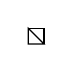
\begin{tikzpicture}[scale=0.2] % adjust scale as needed
      % Bottom triangle
      \draw[]
        (0,0) coordinate (A)
        -- (0,1) coordinate (B)
        -- (1,0) coordinate (C)
        -- cycle;
      % Upper triangle
      \draw[]
        (0,1) coordinate (D)
        -- (1,1) coordinate (E)
        -- (1,0) coordinate (F);
    \end{tikzpicture}
}

\newcommand{\playthumb}[2][]{%
  \begin{tikzpicture}
    % Thumbnail image
    \node[inner sep=0] (img) {\includegraphics[#1]{#2}};
    % Dark circle
    \draw[fill=black!60, draw=white, line width=0.8pt]
      (img.center) circle[radius=0.6cm];
    % Triangle
    \draw[fill=white, draw=none, rounded corners=1.5pt]
      ([xshift=0.34cm]img.center) --
      ([xshift=-0.19cm,yshift=0.3cm]img.center) --
      ([xshift=-0.19cm,yshift=-0.3cm]img.center) -- cycle;
  \end{tikzpicture}%
}

\newcounter{video}
\renewcommand{\thevideo}{Video \arabic{video}}
\newcommand{\videoCaption}[1]{%
  \captionof{video}{#1}%
}

\newcommand{\externalvod}[3]{\movie[externalviewer]{\playthumb[#1]{#3}}{#2}}
\newcommand{\seudoembeddedvod}[3]{\movie[poster, showcontrols]{\playthumb[#1]{#3}}{#2}}

\DeclareRobustCommand{\labelbox}[2][]{%
  % Inline TikZ node; safe in text, math, tabular, makebox, etc.
  \tikz[baseline=(X.base)]\node[annotate box,#1] (X) {#2};%
}
\newcommand{\support}[1]{\text{supp}\left(#1\right)}
\newcommand{\nablaxi}[0]{\nabla_{\boldsymbol{\xi}}}
\newcommand{\deltaxi}[0]{\Delta_{\boldsymbol{\xi}}}
\newcommand{\eunorm}[1]{
  \text{\Large$|\hspace{-0.8mm}|$}\; #1 \;\text{\Large$|\hspace{-0.8mm}|_{\scriptscriptstyle{2}}$}
}

\pgfplotsset{
  colormap={rainbow}{
    rgb255(0.0cm)=(5,97,254);
    rgb255(0.023809523809523808cm)=(5,108,247);
    rgb255(0.047619047619047616cm)=(5,119,239);
    rgb255(0.07142857142857142cm)=(5,130,232);
    rgb255(0.09523809523809523cm)=(5,139,222);
    rgb255(0.11904761904761904cm)=(5,148,212);
    rgb255(0.14285714285714285cm)=(5,157,202);
    rgb255(0.16666666666666666cm)=(5,166,191);
    rgb255(0.19047619047619047cm)=(5,174,179);
    rgb255(0.21428571428571427cm)=(5,183,167);
    rgb255(0.23809523809523808cm)=(5,193,153);
    rgb255(0.2619047619047619cm)=(5,202,140);
    rgb255(0.2857142857142857cm)=(5,211,126);
    rgb255(0.30952380952380953cm)=(5,220,109);
    rgb255(0.3333333333333333cm)=(5,228,91);
    rgb255(0.35714285714285715cm)=(4,237,74);
    rgb255(0.38095238095238093cm)=(69,242,39);
    rgb255(0.40476190476190477cm)=(125,245,28);
    rgb255(0.42857142857142855cm)=(164,249,11);
    rgb255(0.4523809523809524cm)=(194,251,8);
    rgb255(0.47619047619047616cm)=(224,252,5);
    rgb255(0.5cm)=(254,254,3);
    rgb255(0.5238095238095238cm)=(254,243,20);
    rgb255(0.5476190476190477cm)=(254,232,37);
    rgb255(0.5714285714285714cm)=(254,220,55);
    rgb255(0.5952380952380952cm)=(254,208,55);
    rgb255(0.6190476190476191cm)=(254,196,55);
    rgb255(0.6428571428571429cm)=(254,183,55);
    rgb255(0.6666666666666666cm)=(254,171,55);
    rgb255(0.6904761904761905cm)=(254,159,55);
    rgb255(0.7142857142857143cm)=(254,147,55);
    rgb255(0.7380952380952381cm)=(254,132,55);
    rgb255(0.7619047619047619cm)=(254,118,55);
    rgb255(0.7857142857142857cm)=(254,104,55);
    rgb255(0.8095238095238095cm)=(253,84,53);
    rgb255(0.8333333333333334cm)=(251,66,48);
    rgb255(0.8571428571428571cm)=(252,37,53);
    rgb255(0.8809523809523809cm)=(242,29,64);
    rgb255(0.9047619047619048cm)=(230,20,74);
    rgb255(0.9285714285714286cm)=(218,10,84);
    rgb255(0.9523809523809523cm)=(203,11,91);
    rgb255(0.9761904761904762cm)=(189,11,98);
    rgb255(1.0cm)=(174,12,105);
  }
}
\pgfplotsset{
  colormap={fast}{
    rgb255(0.0cm)=(22,47,140);
    rgb255(0.16144cm)=(56,131,180);
    rgb255(0.351671cm)=(128,220,221);
    rgb255(0.501285cm)=(255,255,211);
    rgb255(0.620051cm)=(240,227,138);
    rgb255(0.835408342528245cm)=(191,113,65);
    rgb255(1.0cm)=(142,14,14);
  }
}
\pgfplotsset{
  colormap={rainbow_blended_white}{
    rgb(0cm)=(1, 1, 1);
    rgb(0.17cm)=(0, 0, 1);
    rgb(0.34cm)=(0, 1, 1);
    rgb(0.5cm)=(0, 1, 0);
    rgb(0.67cm)=(1, 1, 0);
    rgb(0.84cm)=(1, 0, 0);
    rgb(1cm)=(0.878431372549, 0, 1);
  }
}
\pgfplotsset{
  colormap={powderbulk}{
    rgb255(0cm)=(224,219,207);
    rgb255(0.499cm)=(224,219,207);
    rgb255(0.501cm)=(107.0,104.0,98.0);
    rgb255(1cm)=(107.0,104.0,98.0);
  }
}

\newcommand{\vcolorbar}[6]{
  \begin{tikzpicture}
    \pgfmathsetmacro{\myheight}{10*#2}
    \pgfmathsetmacro{\widthcolorbar}{#2}
    \pgfmathsetmacro{\cmin}{#3}
    \pgfmathsetmacro{\cmax}{#4}
    \def\extraticks{#6}
    \ifx\extraticks\empty
      \def\ticklist{0,1}
    \else
      \def\ticklist{0,\extraticks,1}
    \fi
    \begin{axis}[
      hide axis,
      scale only axis,
      height=\myheight,
      width=\widthcolorbar,
      colormap name={#1},
      colorbar,
      colorbar style={
        ytick={\ticklist},
        yticklabel pos=right,
        yticklabel style={font=\footnotesize},
        yticklabel={
          \pgfmathparse{\cmin+(\cmax-\cmin)*\tick}\pgfmathprintnumber[precision=1, fixed]{\pgfmathresult}
        },
        ylabel=#5,
        ylabel style={
          at={(0.0,0.5)},
          anchor=south,
          rotate=0,
          font=\footnotesize,
          overlay,
        },
        yticklabel style={
          font=\footnotesize,
          overlay,
        },
        width=\widthcolorbar,
      },
      point meta min=0,
      point meta max=1,
    ]
      % dummy plot just to draw colorbar:
      \addplot [draw=none] coordinates {(0,0) (0,1)};
    \end{axis}
  \end{tikzpicture}
}
\newcommand{\hcolorbar}[6]{
  \begin{tikzpicture}
    \pgfmathsetmacro{\myheight}{#2}
    \pgfmathsetmacro{\widthcolorbar}{10*#2}
    \pgfmathsetmacro{\cmin}{#3}
    \pgfmathsetmacro{\cmax}{#4}
    \def\extraticks{#6}
    \ifx\extraticks\empty
      \def\ticklist{0,1}
    \else
      \def\ticklist{0,\extraticks,1}
    \fi
    \begin{axis}[
      hide axis,
      scale only axis,
      height=\myheight,
      width=\widthcolorbar,
      colormap name={#1},
      colorbar horizontal,
      colorbar style={
        xtick={\ticklist},
        xticklabel pos=left,
        xticklabel style={font=\footnotesize},
        xticklabel={
          \pgfmathparse{\cmin+(\cmax-\cmin)*\tick}\pgfmathprintnumber[precision=1, fixed]{\pgfmathresult}
        },
        xticklabel style={font=\footnotesize},
        xlabel=#5,
        xlabel style={at={(0.5,1.0)}, rotate=0, anchor=south, font=\footnotesize},,
        width=\widthcolorbar,
      },
      point meta min=0,
      point meta max=1,
    ]
      % dummy plot just to draw colorbar:
      \addplot [draw=none] coordinates {(0,0) (0,1)};
    \end{axis}
  \end{tikzpicture}
}


\pgfplotsset{
  convplotstyle/.style={
    clip=true,
    xlabel={$\Delta t_{f} [T_{hs}]$},
    ylabel={$||u_h - u_{ex}||_2$},
    grid=major,
    xtick={1,0.5,0.25,0.125,0.0625},
    xticklabels={$1$,$\tfrac{1}{2}$,$\tfrac{1}{4}$,$\tfrac{1}{8}$,$\tfrac{1}{16}$},
    x dir=reverse,
    scale only axis,
  },
  oscillationstyle/.style={
    clip=true,
    enlargelimits=false,
    ymin=25.0,
    ymax=2400.0,
    grid=major,
    ytick={25,400,900,1300,1625,1900,2300},
    cycle list={
      {blue,solid},
      {red,solid},
      {brown,solid},
      {blue,  densely dashdotted},
      {red,   densely dashdotted},
      {brown, densely dashdotted}
    },
    xlabel={$x$},
    x unit=\si{\mm},
    ylabel={$T$},
    y unit=\si{\celsius},
    legend cell align=left,
    legend image post style={xscale=0.8},
    %legend style={draw=none, fill=none, font=\small},
    legend style={font=\footnotesize},
    tick label style={font=\footnotesize},
    ylabel style={font=\footnotesize},
    xlabel style={font=\footnotesize},
  },
  uhnstyle/.style={mark=none, thick, blue},
  uhnpstyle/.style={mark=none, thick, purple},
  substepstyle/.style={mark=none, thick, black},
  correctstyle/.style={mark=none, thick, green, dashdotted},
  truncatedddstyle/.style={
    clip=true,
    enlargelimits=false,
    ymin=25.0,
    ymax=2400.0,
    xmin=-1.0,
    xmax=0.6,
    grid=major,
    ytick={25,400,900,1300,1900,2300},
    xlabel={$x$},
    x unit=\si{\mm},
    ylabel={$T$},
    ylabel style={at={(axis description cs:-0.2,1.03)}, anchor=south, rotate=-90},
    y unit=\si{\celsius},
    legend cell align=left,
    legend image post style={xscale=0.8},
    %legend style={draw=none, fill=none, font=\small},
    trim axis left,
    scale only axis,
    legend style={font=\footnotesize, text opacity=1.0, fill opacity=0.6},
  },
  meltpoolstyle/.style={
    width=1.0\linewidth,
    grid=major,
    legend cell align=left,
    legend style={font=\footnotesize},
    tick label style={font=\footnotesize},
    cycle list name=color list,
    unit vector ratio=1 1,
    extra x ticks={50},
    extra x tick labels={},
  },
  powderStyle/.style={black, thick, mark=square},
  bulkStyle/.style={blue, thick, mark=diamond}
}

\newcommand{\gammafs}{
  \pgfkeysgetvalue{/pgfplots/ymin}\myymin
  \pgfkeysgetvalue{/pgfplots/ymax}\myymax
  \draw[densely dashed, very thin] (-0.15313, \myymin) -- (-0.15313, \myymax)
    node [pos=0.2, anchor=east] {$\Gamma_{fs}$};
}


\begin{document}

  \begin{frame}[titleslide]
    \titlepage
  \end{frame}

  \setbeamertemplate{frame footer}{\qquad Computational strategies for time-accurate simulation of part-scale \footlineHl{LPBF}}
  \section{Introduction}
    \subsection{LPBF}
      \begin{frame}[sectionslide]
  \begin{center}
    \video<1>[above,autoplay,height=0.7,aspectratio=359/208,fit=contain]
\at (0.5,0.15) {videos/lpbf.mp4}
    % \begin{tikzpicture}[remember picture,overlay]
    %    \node[anchor=south west, inner sep=0pt] at (current page.south west) {%
    %      \movie[autostart] {\includegraphics[width=0.8\textwidth]{thumbnail-lpbf-section.png}}{videos/lpbf.mp4}%
    %    };
    % \end{tikzpicture}
  \end{center}
\end{frame}

\begin{frame}
  \frametitle{{LPBF}}
  \framesubtitle{MAM technology}
  Also known as PBF-LB/M (ISO nomenclature), one of the
  main Metal Additive Manufacturing (MAM) technologies

  \begin{figure}
    \begin{subfigure}[t]{0.32\textwidth}
      \centering
      \includegraphics[width=\linewidth]{waam.jpg}
      \textbf{Wire Arc Additive Manufacturing
      (\raisebox{-5pt}{\includegraphics[height=16pt]{waam-comic-effect.png}})}
    \end{subfigure}%
    \hfill
    \begin{subfigure}[t]{0.32\textwidth}
      \centering
      \includegraphics[width=\linewidth]{ded.jpg}
      \textbf{Directed Energy Deposition (DED)}
    \end{subfigure}%
    \hfill
    \begin{subfigure}[t]{0.32\textwidth}
      \centering
      \includegraphics[width=\linewidth]{lpbf.png}
      \textbf{Laser Powder Bed Fusion (LPBF)}
    \end{subfigure}
  \end{figure}
\end{frame}

\begin{frame}
  \frametitle{LPBF}
  % \framesubtitle{How does it work?}
  \begin{center}
    \video<1>[above,autoplay,height=0.7,aspectratio=16/9,fit=fill,controls]
\at (0.5,0.1) {videos/Build_chamber_process_animation.webm}
  \end{center}
\end{frame}

\begin{frame}
  \frametitle{{LPBF}}
  \framesubtitle{Fast, small, precise}

  \begin{table}
    \centering
    \begin{tabular}{l
      S
      S
      S }
      \toprule
      & {Radius $R$} 
      & {Speed $V$} 
      & {Power $P$} \\
      \midrule
      WAAM 
        & \qtyrange[]{2}{4}{\milli\meter}
        & \qtyrange[]{3}{10}{\milli\meter\per\second}
        & \qtyrange[]{5}{15}{\kilo\watt} \\
      DED 
        & \qtyrange[]{0.5}{1.5}{\milli\meter}
        & \qtyrange[]{5}{20}{\milli\meter\per\second}
        & \qtyrange[]{1}{4}{\kilo\watt} \\
      LPBF 
        & \qtyrange[]{25}{100}{\micro\meter}
        & \qtyrange[]{400}{1400}{\milli\meter\per\second}
        & \qtyrange[]{0.2}{1}{\kilo\watt} \\
      \bottomrule
    \end{tabular}
    \caption{Characteristic heat source parameters for the main MAM technologies.}
  \end{table}
  \vspace{-4mm}
  % LPBF offers a finer resolution and smoother surface finish,
  % but it is limited to smaller parts.
  \begin{figure}
    \centering
    \begin{subfigure}[t]{0.48\textwidth}
      \centering
      \includegraphics[width=0.74\linewidth]{waam-example.jpg}\\
      {\scriptsize WAAM: large parts (> \qty{1}{\meter}), coarse features.}
    \end{subfigure}%
    \hfill
    \begin{subfigure}[t]{0.48\textwidth}
      \centering
      \includegraphics[width=0.55\linewidth]{lpbf-fine.png}\\
      {\scriptsize LPBF: small part (< \qty{1}{\meter}), fine features.}
    \end{subfigure}
  \end{figure}

\end{frame}


    \setbeamertemplate{frame footer}{Computational strategies for time-accurate \footlineHl{simulation} of \footlineHl{part-scale} LPBF}
    \subsection{Multiscale application}
      \begin{frame}
  \frametitle{LPBF}
  \framesubtitle{Extremely multiscale}
  LPBF is an \textit{extremely multiscale} application \citep{hodge2021}.\\
  Let's quantify this statement:
  \begin{itemize}
    \item The \textbf{smallest} spatial and temporal \textbf{scales} are governed by the
      \textbf{heat source}, characterized by its radius $\mathbf{R}$ and by
      the time it takes to travel one radius,
      \[
        \mathbf{T_{hs}} := \frac{R}{V}.
      \]
    \item The \textbf{largest} spatial and temporal \textbf{scales} are set
      by the \textbf{part} and the printer.
      We choose here the characteristic part length $\mathbf{L_{part}}$ and
      the net printing time $\mathbf{T_{print}}$, i.e. the cumulative
      laser-on time.
  \end{itemize}
\end{frame}

\begin{frame}
  \frametitle{LPBF}
  \framesubtitle{Extremely multiscale}
  \centering
  \begin{minipage}{0.59\textwidth}
    \begin{figure}[ht]
      \def\svgwidth{0.84\columnwidth}
      \import{./figures/cube-example}{cube-scan-schematic.pdf_tex}
      \caption{Cube scan path of \textbf{side length} $L$, \textbf{layer thickness} $t$
      and \textbf{hatch spacing} $h$.}
    \end{figure}
  \end{minipage}%
  \hfill%
  \begin{minipage}{0.38\textwidth}
    Consider printing a cube of side length $L$.
    The ratio of volume scales is
    $$
    \frac{L^3}{R^3}
    $$
    Let's compute the time scale ratio.
    Assume $t~=~h~=~R$ for simplicity, so that
    $$N_{layers} = N_{hatches\\/layer} = \frac{L}{R}$$
  \end{minipage}
\end{frame}

\begin{frame}
  \frametitle{LPBF}
  \framesubtitle{Extremely multiscale}
  For this simple geometry, the net print time is
  \begin{gather*}
    T_{print} = N_{hatches} \cdot T_{hatch} = N_{layers} \cdot N_{hatches/layer} \cdot T_{hatch}\\
    T_{hatch} = \frac{L}{V}\\
    \implies
    T_{print} = \frac{L}{R} \cdot \frac{L}{R} \cdot \frac{L}{V} = \frac{L^2}{R^2} \cdot \frac{L}{V} = \frac{L^3}{R^2 V}
  \end{gather*}
  Therefore, the time scale disparity is
  $$
  \frac{T_{print}}{T_{hs}} = \frac{L^3}{R^2 V} \cdot \frac{V}{R} = \left(\frac{L}{R}\right)^3
  $$
\end{frame}

\begin{frame}
  \frametitle{LPBF}
  \framesubtitle{Multiphysics}
  \begin{figure}
    \centering
    \includegraphics[height=0.8\textheight]{bayat2021.png}
    \caption{Relevant physics at melt-pool and part scales \citep{bayat2021}.}
    \label{fig:bayat2021}
  \end{figure}
\end{frame}

\begin{frame}
  \frametitle{Part-scale simulation}
  \framesubtitle{Why?}

  LPBF is both \textbf{extremely multiscale} and a \textbf{multiphysics} application.
  Despite this complexity, predictions are required at the \textbf{part scale}.

  \vspace{0.5em}
  Part-scale simulation aims to:
  \begin{itemize}
    \item Reduce costly experimental trial-and-error
    \item Predict residual stresses and part distortions
    \item Link thermal history to microstructure features
    \item Enable process-parameter optimization
    \item Shorten the design-to-manufacturing cycle
  \end{itemize}
\end{frame}

\begin{frame}
  \frametitle{Part-scale simulation}
  \framesubtitle{Problem statement}
  \begin{figure}[ht]
    \def\svgwidth{0.9\columnwidth}
    \hspace{-6mm}
    \import{./figures/lpbf_schematic}{schematic.pdf_tex}
    \caption{Schematic of the LPBF computational domain 
    $\Omega(t)$, encompassing the bulk (part and substrate) and powder bed regions,
    together with the applied heat source and convective/radiative heat losses.
  }
  \end{figure}
\end{frame}

\begin{frame}
  \frametitle{Part-scale simulation}
  \framesubtitle{PDE}
  {\small
  Define the extended temperature and liquid fraction fields
  \begin{equation*}
    T_e\dependson{\mathbf{x}, t} =
    \begin{cases}
      T\dependson{\mathbf{x}, t} & \mathbf{x} \in \overline{\Omega}(t)\\
      T_{dep} & \mathbf{x} \in \overline{\Omega}(t_{final}) \setminus \overline{\Omega}(t)
    \end{cases}
    \qquad
    f_{l,\; e}\dependson{\mathbf{x}, t} = f_l(T_e\dependson{\mathbf{x}, t})
  \end{equation*}
  where $T_{dep}$ is the deposition temperature.\\
  Find $T : \Omega(t) \times [0, T_{\text{final}}] \to \mathbb{R}$ such that
  \begin{align}
    \label{eq:original_pde}
    \rho c_p \partial_t T_e + \rho L \partial_t f_{l,\; e} - k \Delta T
    &= r\dependson{\mathbf{x}, t} &&\forall \mathbf{x} \in \Omega(t)\\
    \notag
    - k \partial_n T &= h_{conv} (T - T_{\text{env}}) + \varepsilon \sigma (T^4 - T_{\text{env}}^4) &&\forall \mathbf{x} \in \partial \Omega(t)\\
    \notag
    T\dependson{\mathbf{x}, 0} &= T_0 \qquad &&\forall \mathbf{x} \in \Omega(0)
  \end{align}
  }
    \todo{Comment on phase change treatment here}
\end{frame}

\begin{frame}
  \frametitle{Part-scale simulation}
  \framesubtitle{Discretization}
    Multiply \cref{eq:original_pde}
    by $\phi \in V_T(t) = H^{1}\left(\Omega(t)\right)$;
    integrate over $\Omega\dependson{t}$;
    apply integration by parts on the diffusion term; insert BCs;
    apply BDF1
    {\small
    \begin{gather*}
      \label{eq:weak_heat}
      \int_{\Omega} \phi \rho \left({c_p \frac{T^{n+1} - T^n}{\Delta t} + L \frac{f_l(T^{n+1}) - f_l(T^n)}{\Delta t}}\right)
      + \int_{\Omega} \nabla \phi \cdot \left(k \nabla T\right)\\
      \notag
      \forall \phi \in V_T(t) \hspace{1cm}
      \;=\; \int_{\Omega} \phi r
      + \int_{\partial \Omega} \phi \left({h_{\text{conv}} \left( T - T_{\text{env}} \right)
      + \varepsilon \sigma \left( {T}^4 - T_{\text{env}}^4 \right)}\right)
    \end{gather*}
    }
\end{frame}

\begin{frame}
  \frametitle{Part-scale simulation}
  \framesubtitle{Discretization}
  \begin{figure}
    \begin{subfigure}[t]{0.30\textwidth}
      \includegraphics[width=\textwidth]{schematic_melting/0.png}
      \caption{Bare substrate below an inactive powder layer.}
      \label{fig:refModelBareSubstrate}
    \end{subfigure}\hfill%
    \begin{subfigure}[t]{0.30\textwidth}
      \includegraphics[width=\textwidth]{schematic_melting/1.png}
      \caption{A powder layer is activated during a recoating step.}
      \label{fig:powderLayer}
    \end{subfigure}\hfill%
    \begin{subfigure}[t]{0.30\textwidth}
      \includegraphics[width=\textwidth]{schematic_melting/2.png}
      \caption{After a heating step, elements whose average temperature
      surpasses $T_m$ are set to bulk.}
      \label{fig:activPhaseChange3}
    \end{subfigure}\hfill%
    \caption{Illustration of deposition and melting processes.\qquad
      \legendpowderbulk{}
    }
    \label{fig:activPhaseChange}.
  \end{figure}
  Same treatment of phase change as in \citep{kollmannsberger2018}
  \todo{Maybe remove this slide, contradicting legend on next slide?}
\end{frame}

\begin{frame}
  \frametitle{Part-scale simulation}
  \framesubtitle{Demo video}

  \begin{figure}
    \video<1>[above,height=0.7,aspectratio=62/27,fit=fill,controls]
  at (0.5,0.18) {videos/2dlpbf_2d_lpbf_ref.mp4}
    \vspace{0.7\pageheight+3pt}
    \videoCaption{
      Demo simulation of 2D LPBF with element activation.\\
      Wireframe elements (\;\wireframeTriangle{}) correspond to powder region.
    }
  \end{figure}

\end{frame}

\begin{frame}
  \frametitle{Part-scale simulation}
  \framesubtitle{Impossible}
  Previous slide: ``uniform'' mesh in part and powder region.
  Recall the volume scale ratio;
  In 3D, we would need
  \begin{equation}
    \label{eq:num_elements_uniform_mesh}
    \text{\# elements} = \mathcal{O}\left(\frac{L^3}{R^3}\right)
  \end{equation}
  to resolve the heat source throughout the print.

  In practice, no one uses uniform meshes for LPBF simulation;
  \textbf{AMR} is regarded as the \textbf{de facto standard}.
\end{frame}

\begin{frame}
  \frametitle{Part-scale simulation}
  \framesubtitle{Impossible}
  But what about time-steps?
  The interval of interest is $]0, T_{final}[$ with
  $$
  T_{final} = T_{print} + T_{cool}
  $$
  i.e. the net printing time plus cooling.
  The time scale disparity requires again \cref{eq:num_elements_uniform_mesh} time-steps
  \begin{gather}
    \label{eq:num_timesteps_uniform_mesh}
    \text{\# time-steps} > \frac{T_{print}}{T_{hs}} = \mathcal{O}\left(\frac{L^3}{R^3}\right)\\
  \end{gather}
  when discretizing with \textbf{uniform time-steps}.
\end{frame}

\begin{frame}
  \frametitle{Part-scale simulation}
  \framesubtitle{Impossible}
  Intuitively, if we don't respect the constraint
  \begin{equation}
    \label{eq:origconstraint}
    \Delta t \leq T_{hs}
  \end{equation}
  , we won't resolve the motion of the heat source.\\
  In practice, that's indeed what happens:
  if the time-step is larger than $T_{hs}$ i.e. the heat source
  travels more than $1 R$ per time-step,
  it skips over parts of the domain,
  and generates artificial temperature spikes.
  \begin{figure}
    \begin{subfigure}[t]{0.49\textwidth}
      \includegraphics[width=\textwidth]{timestep-2ths/1R.png}
      \caption{$\Delta t = 1 T_{hs}$}
      \label{fig:spots1R}
    \end{subfigure}
    \begin{subfigure}[t]{0.49\textwidth}
      \includegraphics[width=\textwidth]{timestep-2ths/2R.png}
      \caption{$\Delta t = 2 T_{hs}$}
      \label{fig:spots2R}
    \end{subfigure}
    % \caption{2D heating track example with admissible and inadmissible
    % time-step sizes according to inequality \eqref{eq:origconstraint}.}
    % \label{fig:spots}
  \end{figure}
\end{frame}

\begin{frame}
  \frametitle{Part-scale simulation}
  \framesubtitle{Impossible}
  So \eqref{eq:num_timesteps_uniform_mesh} is indeed a \textbf{lower bound} on the number of time-steps
  when using uniform time-stepping.

  \underline{Bad news:}
  \begin{itemize}
    \item \textbf{Uniform time-stepping} is the \textbf{de facto standard} in LPBF simulation.
    \item Some references require time-steps much smaller than $T_{hs}$
      to ensure stability and accuracy \citep{hodge2014, hodge2021, elahi2025}.
  \end{itemize}
  There are basically 4 (!) groups in the world that can run simulations in the order of $\mathcal{O}(10 \unit{\milli\meter})$:
  Pittsburgh, Northwestern, LLNL, TUM.\\
  Decimeter-scale parts are currently unfeasible.
  \todo{Expand}
\end{frame}



    \setbeamertemplate{frame footer}{Computational strategies for \footlineHl{time-accurate} simulation part-scale LPBF}
    \subsection{Part-scale simulation}
      \begin{frame}
  \frametitle{Part-scale simulation}
  \framesubtitle{Why?}

  LPBF is both \textbf{extremely multiscale} and a \textbf{multiphysics} application.
  Despite this complexity, predictions are required at the \textbf{part scale}.

  \vspace{0.5em}
  Part-scale simulation aims to:
  \begin{itemize}
    \item Reduce costly experimental trial-and-error
    \item Predict residual stresses and part distortions
    \item Link thermal history to microstructure features
    \item Enable process-parameter optimization
    \item Shorten the design-to-manufacturing cycle
  \end{itemize}
\end{frame}

\begin{frame}
  \frametitle{Part-scale simulation}
  \framesubtitle{Problem statement}
  \begin{figure}[ht]
    \def\svgwidth{0.9\columnwidth}
    \hspace{-6mm}
    \import{./figures/lpbf_schematic}{schematic.pdf_tex}
    \caption{Schematic of the LPBF computational domain 
    $\Omega(t)$, encompassing the bulk (part and substrate) and powder bed regions,
    together with the applied heat source and convective/radiative heat losses.
  }
  \end{figure}
\end{frame}

\begin{frame}
  \frametitle{Part-scale simulation}
  \framesubtitle{PDE}
  {\small
  Define the extended temperature and liquid fraction fields
  \begin{equation*}
    T_e\dependson{\mathbf{x}, t} =
    \begin{cases}
      T\dependson{\mathbf{x}, t} & \mathbf{x} \in \overline{\Omega}(t)\\
      T_{dep} & \mathbf{x} \in \overline{\Omega}(t_{final}) \setminus \overline{\Omega}(t)
    \end{cases}
    \qquad
    f_{l,\; e}\dependson{\mathbf{x}, t} = f_l(T_e\dependson{\mathbf{x}, t})
  \end{equation*}
  where $T_{dep}$ is the deposition temperature.\\
  Find $T : \Omega(t) \times [0, T_{\text{final}}] \to \mathbb{R}$ such that
  \begin{align}
    \label{eq:original_pde}
    \rho c_p \partial_t T_e + \rho L \partial_t f_{l,\; e} - k \Delta T
    &= r\dependson{\mathbf{x}, t} &&\forall \mathbf{x} \in \Omega(t)\\
    \notag
    - k \partial_n T &= h_{conv} (T - T_{\text{env}}) + \varepsilon \sigma (T^4 - T_{\text{env}}^4) &&\forall \mathbf{x} \in \partial \Omega(t)\\
    \notag
    T\dependson{\mathbf{x}, 0} &= T_0 \qquad &&\forall \mathbf{x} \in \Omega(0)
  \end{align}
  }
    \todo{Comment on phase change treatment here}
\end{frame}

\begin{frame}
  \frametitle{Part-scale simulation}
  \framesubtitle{Discretization}
    Source-based latent heat treatment of \cite{celentano1994}:
    $f_l(T)$ is directly discretized in time.
    \begin{figure}
      \centering
      \begin{subfigure}[t]{0.33\textwidth}
        \begin{tikzpicture}
        \begin{axis}[
            xmin=-0.1, xmax=1.1,
            ymin=+0, ymax=1.1,
            axis lines=center,
            axis on top=true,
            ytick={0, 1},
            xtick={0.05, 0.95},
            xticklabels={$T_s$, $T_l$},
            domain=-0.1:1.1,
            ylabel=$f_l$,
            xlabel=$T$,
            %legend style={at={(0.03,0.5)},anchor=west},
            height=0.4\pageheight
            ]

            \def\Ts{0.05}
            \def\Tl{0.95}
            \newcommand{\flalpha}[1]{2*#1/(\Tl - \Ts)}
            \newcommand{\fl}[1]{
              0.5*(tanh(\flalpha{#1}*(\x - 0.5))+1)
            }
            \addplot+ [mark=none, ultra thick, smooth] {\fl{1}};
            \addplot+ [mark=none, ultra thick, smooth] {\fl{2}};
            \addplot+ [mark=none, ultra thick, smooth] {\fl{4}};
            
            %% Add the asymptotes
            \draw [blue, dotted, thick] (axis cs:+1.1,+1)-- (axis cs:0,+1);
        \end{axis}
        \end{tikzpicture}
      \end{subfigure}%
      \hfill
      \begin{subfigure}[t]{0.33\textwidth}
        \begin{tikzpicture}
        \begin{axis}[
            xmin=-0.1, xmax=1.1,
            ymin=+0, ymax=4.5,
            axis lines=center,
            axis on top=true,
            ytick={0},
            xtick={0.05, 0.95},
            xticklabels={$T_s$, $T_l$},
            domain=-0.1:1.1,
            ylabel=$f_l'$,
            legend style={at={(0.7,0.8)},anchor=west},
            height=0.4\pageheight
            ]

            \def\Ts{0.05}
            \def\Tl{0.95}
            \newcommand{\flalpha}[1]{2*#1/(\Tl - \Ts)}
            \newcommand{\flp}[1]{
              \flalpha{#1}/2*(1 - (tanh(\flalpha{#1}*(\x - 0.5)))^2)
            }
            \addplot+ [mark=none, ultra thick, smooth] {\flp{1}};
            \addlegendentry{$S = 1$}                
            \addplot+ [mark=none, ultra thick, smooth] {\flp{2}};
            \addlegendentry{$S = 2$}                
            \addplot+ [mark=none, ultra thick, smooth] {\flp{4}};
            \addlegendentry{$S = 4$}
            
        \end{axis}
        \end{tikzpicture}
      \end{subfigure}%
      \hfill
      \begin{subfigure}[t]{0.33\textwidth}
        \begin{tikzpicture}
        \begin{axis}[
            xmin=-0.1, xmax=1.1,
            ymin=-4, ymax=4,
            axis lines=center,
            axis on top=true,
            ytick={0},
            xtick={0.05, 0.95},
            xticklabels={$T_s$, $T_l$},
            domain=-0.1:1.1,
            ylabel=$f_l''$,
            height=0.4\pageheight
            ]

            \def\Ts{0.05}
            \def\Tl{0.95}
            \newcommand{\flalpha}[1]{2*#1/(\Tl - \Ts)}
            \newcommand{\flpp}[1]{
              \flalpha{#1}^2*tanh(\flalpha{#1}*(\x - 0.5))*((tanh(\flalpha{#1}*(\x - 0.5)))^2 - 1)
            }
            \addplot+ [mark=none, ultra thick, smooth] {\flpp{1}};
            \addplot+ [mark=none, ultra thick, smooth] {\flpp{2}};
            \addplot+ [mark=none, ultra thick, smooth] {\flpp{4}};
            
        \end{axis}
        \end{tikzpicture}
      \end{subfigure}
      \caption{Liquid fraction $f_l$ and derivatives.}
      \label{fig:fl_fld_fldd}
    \end{figure}
    Multiply \cref{eq:original_pde}
    by $\phi \in V_T(t) = H^{1}\left(\Omega(t)\right)$;
    integrate over $\Omega\dependson{t}$;
    apply integration by parts on the diffusion term; insert BCs;
    apply BDF1
    {\small
    \begin{gather*}
      \label{eq:weak_heat}
      \int_{\Omega} \phi \rho \left({c_p \frac{T^{n+1} - T^n}{\Delta t} + L \frac{f_l(T^{n+1}) - f_l(T^n)}{\Delta t}}\right)
      + \int_{\Omega} \nabla \phi \cdot \left(k \nabla T\right)\\
      \notag
      \forall \phi \in V_T(t) \hspace{1cm}
      \;=\; \int_{\Omega} \phi r
      + \int_{\partial \Omega} \phi \left({h_{\text{conv}} \left( T - T_{\text{env}} \right)
      + \varepsilon \sigma \left( {T}^4 - T_{\text{env}}^4 \right)}\right)
    \end{gather*}
    }

\end{frame}

\begin{frame}
  \frametitle{Part-scale simulation}
  \framesubtitle{Discretization}
  \begin{figure}
    \begin{subfigure}[t]{0.33\textwidth}
      \includegraphics[height=0.35\pageheight]{schematic_melting/0.png}
      \caption{Bare substrate below an inactive powder layer.}
      \label{fig:refModelBareSubstrate}
    \end{subfigure}\hfill%
    \begin{subfigure}[t]{0.33\textwidth}
      \includegraphics[height=0.35\pageheight]{schematic_melting/1.png}
      \caption{A powder layer is activated during a recoating step.}
      \label{fig:powderLayer}
    \end{subfigure}\hfill%
    \begin{subfigure}[t]{0.33\textwidth}
      \includegraphics[height=0.35\pageheight]{schematic_melting/2.png}
      \caption{After a heating step, elements whose average temperature
      surpasses $T_m$ are set to bulk.}
      \label{fig:activPhaseChange3}
    \end{subfigure}\hfill%
    \caption{Illustration of deposition and melting processes.\qquad
      \legendpowderbulk{}
    }
    \label{fig:activPhaseChange}.
  \end{figure}
  Same treatment of phase change as in \citep{kollmannsberger2018}
\end{frame}

\begin{frame}
  \frametitle{Part-scale simulation}
  \framesubtitle{Demo video}

  \begin{figure}
    \video<1>[above,height=0.7,aspectratio=62/27,fit=fill,controls]
  at (0.5,0.18) {videos/2dlpbf_2d_lpbf_ref.mp4}
    \vspace{0.7\pageheight+3pt}
    \videoCaption{
      Demo simulation of 2D LPBF with element activation.\\
      Wireframe elements (\;\wireframeTriangle{}) correspond to powder region.
    }
  \end{figure}

\end{frame}


  \setbeamertemplate{frame footer}{\footlineHl{Computational strategies for time-accurate simulation part-scale LPBF}}
  \section{Objectives}
    \begin{frame}
  \frametitle{Problematic}
  \begin{itemize}
    \item AMR is regarded as necessary for part-scale LPBF simulation
      to adress spatial scale disparity.
    \item The time scale disparity is \textbf{equally} severe,
      yet uniform-time stepping is the standard.
  \end{itemize}
  $\implies$ Largely overlooked challenge:
  reduce the number of global time-steps required
  in part-scale LPBF simulation
  while retaining time-accuracy.
\end{frame}

\begin{frame}
  \frametitle{Objectives of this work}
  \begin{itemize}
    \item
      Review existing methods for addressing time-stepping
      challenges in MAM.
    \item
      Explore novel methods for reducing the number of time-steps
      required in LPBF modeling.
    \item
      Validate the proposed methods on realistic
      test cases.
    \item
      Validate the underlying physical models
      and numerical methods against experimental data.
    \item
      Provide realistic speedup estimates and practical implementation guidelines
      for the proposed methods.
    \item Ensure open science and reproducibility.
  \end{itemize}
\end{frame}



  \setbeamertemplate{frame footer}{}
  \begin{frame}
    \centering
    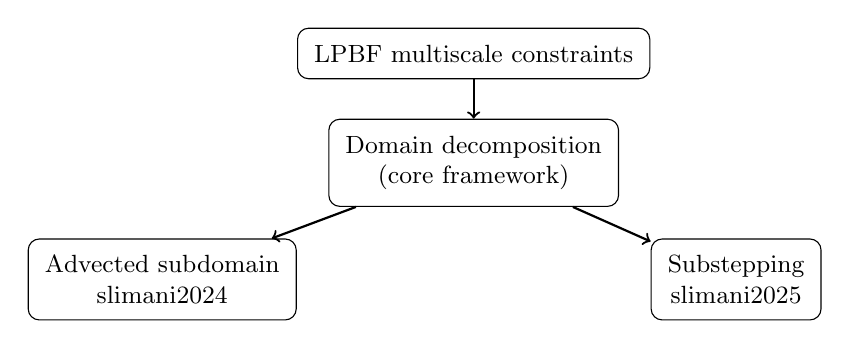
\begin{tikzpicture}[
      font=\small,
      box/.style={draw, rounded corners, align=center, inner sep=6pt},
      arr/.style={->, thick}
    ]

    \node[box] (ms) {LPBF multiscale constraints};

    \node[box, below=5mm of ms] (dd) {Domain decomposition\\(core framework)};

    \node[box, below left=4mm and 4mm of dd] (as) {Advected subdomain\\\citep{slimani2024}};

    \node[box, below right=4mm and 4mm of dd] (ss) {Substepping\\\citep{slimani2025}};

    \draw[arr] (ms) -- (dd);
    \draw[arr] (dd) -- (as);
    \draw[arr] (dd) -- (ss);

    \end{tikzpicture}
  \end{frame}
  \section{Domain decomposition}
    \begin{frame}
  \centering
  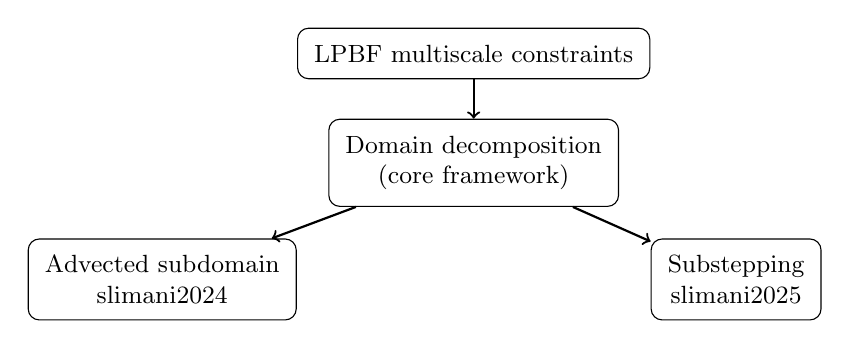
\begin{tikzpicture}[
    font=\small,
    box/.style={draw, rounded corners, align=center, inner sep=6pt},
    arr/.style={->, thick}
  ]

  \node[box] (ms) {LPBF multiscale constraints};

  \node[box, below=5mm of ms] (dd) {Domain decomposition\\(core framework)};

  \node[box, below left=4mm and 4mm of dd] (as) {Advected subdomain\\\citep{slimani2024}};

  \node[box, below right=4mm and 4mm of dd] (ss) {Substepping\\\citep{slimani2025}};

  \draw[arr] (ms) -- (dd);
  \draw[arr] (dd) -- (as);
  \draw[arr] (dd) -- (ss);

  \end{tikzpicture}
\end{frame}

\begin{frame}
  \frametitle{Domain decomposition}
  \framesubtitle{Basics}
  We've established that the part-scale build is driven
  by the motion of a very localized heat source.

  What if we treat differently this region aka the Heat Affected Zone (HAZ)?

  We will do so via \textbf{domain decomposition} (DD).

  Let $\Omega_1$ and $\Omega_2$ be a non-overlapping decomposition of
  the domain $\Omega = \Omega_1 \sqcup \Omega_2$ such that
  $\Omega_1$ contains the HAZ;
  we will pose different problems in $\Omega_1$ and $\Omega_2$
  and enforce \textbf{transmission conditions} at the interface
  $\Gamma = \partial \Omega_1 \cap \partial \Omega_2$
\end{frame}

\begin{frame}
  \frametitle{Domain decomposition}
  \framesubtitle{Basics}
\begin{figure}
  \centering
  \def\svgwidth{1.0\columnwidth}
  \import{figures/transmission_conds/}{drawing.pdf_tex}
  \caption{Non-overlapping DD schematic for a welding problem. $\Omega_1$ and $\Omega_2$
  cover the HAZ and underlying substrate, respectively. Transmission conditions
  must be satisfied at the interface $\Gamma = \partial \Omega_1 \cap \partial \Omega_2$.
  Admissible and inadmissible transmission conditions are shown in the miniature plots,
  which represent temperature fields across $\Gamma$.
  }
  \label{fig:transmission_conditions}
\end{figure}
\end{frame}

\begin{frame}
  \frametitle{Domain decomposition}
  \framesubtitle{Basics}
  Consider the linear heat equation with Dirichlet boundary conditions.
  Solve for $T_i$ in each subdomain $\Omega_i$:
  \begin{equation}
  \label{eq:lproblem}
  \left\{
  \begin{aligned}
    \partial_t T_i - \alpha \Delta T_i &= r && \forall \mathbf{x} \in \Omega_i\\
    T_i(\mathbf{x}, t) &= T_d && \forall \mathbf{x} \in \partial \Omega_{D,i}\\
    \mathcal{I}_i \left(T_i, T_j\right) &= 0 && \forall \mathbf{x} \in \Gamma, \enskip i \neq j
  \end{aligned}
  \right.
  \end{equation}
  This is equivalent to solving the original problem in $\Omega$ given
  that the \textbf{transmission conditions}
  are satisfied
  \begin{equation}
    \label{eq:interface_eq_conditions}
    \begin{cases}
      \mathcal{I}_1(T_1, T_2) = 0\\
      \mathcal{I}_2(T_1, T_2) = 0
    \end{cases}
    \iff
    \begin{cases}
      T_1 = T_2\\
      k_1 \partial_n T_1 = k_2 \partial_n T_2
    \end{cases}
    \qquad
    \qquad
    \forall \mathbf{x} \in \Gamma
  \end{equation}
\end{frame}

\begin{frame}
  \frametitle{Domain decomposition}
  \framesubtitle{Basics}
  Any linearly independent combination of \eqref{eq:interface_eq_conditions}
  lays a valid pair of subproblems on $\Omega_1$ and $\Omega_2$
  {\small
  \begin{equation}
    \label{eq:lp1}
    \left\{
    \begin{aligned}
      \rho c_p \partial_t T_1 - k \Delta T_1 &= r && \text{ in } \Omega_1\\
      T_1 &= T_d && \text{ in } \partial \Omega_{D,1}\\
      \gamma_1 T_1 + \eta_1 k_1 \frac{\partial T_1}{\partial n_1} &= \gamma_1 T_2 + \eta_1 k_2 \frac{\partial T_2}{\partial n_1} && \text{ in } \Gamma
    \end{aligned}
    \right.
  \end{equation}
  \begin{equation}
    \label{eq:lp2}
    \left\{
    \begin{aligned}
      \rho c_p \partial_t T_2 - k \Delta T_2 &= r && \text{ in } \Omega_2\\
      T_2 &= T_d && \text{ in } \partial \Omega_{D,2}\\
      \gamma_2 T_2 + \eta k_2 \frac{\partial T_2}{\partial n_2} &= \gamma_2 T_2 + \eta_2 k_2 \frac{\partial T_2}{\partial n_2} && \text{ in } \Gamma
    \end{aligned}
    \right.
  \end{equation}
  }
  \begin{itemize}
    \item $\gamma_1 = \eta_2 \neq 0$ and $\gamma_2 = \eta_1 = 0 \longrightarrow\;$ Dirichlet-Neumann

    \item $\gamma_i \neq 0$ and $\eta_i \neq 0 \longrightarrow\;$ Robin-Robin

    \item $\gamma_1 \neq 0$, $\eta_1 = 0$, $\gamma_2 \neq 0$ and $\eta_2 \neq 0
      \longrightarrow\;$ Dirichlet-Robin
  \end{itemize}
\end{frame}

\begin{frame}
  \frametitle{Domain decomposition}
  \framesubtitle{Basics}
  Assuming steady-state and applying FEM discretization
  on both subdomains, we obtain the following
  monolithic system:
  \renewcommand{\arraystretch}{1.2} % increases spacing (default is 1.0)
  \begin{equation}
    \label{eq:monolithic}
    \begin{pmatrix}
      \mathbf{A}_{11} & \mathbf{A}_{1\Gamma_1} & \cdot & \cdot\\
      \mathbf{A}_{\Gamma_1 1} & \mathbf{A}_{\Gamma_1 \Gamma_1} + \mathbf{R}_{11} & \cdot & \mathbf{R}_{12}\\
      \cdot & \cdot & \mathbf{A}_{22} & \mathbf{A}_{2\Gamma_2}\\
      \cdot & \mathbf{R}_{21} & \mathbf{A}_{\Gamma_2 2} & \mathbf{A}_{\Gamma_2 \Gamma_2} + \mathbf{R}_{22}
    \end{pmatrix}
    \begin{pmatrix}
      \mathbf{T}_1\\
      \mathbf{T}_{\Gamma_1}\\
      \mathbf{T}_2\\
      \mathbf{T}_{\Gamma_2}
    \end{pmatrix}
    =
    \begin{pmatrix}
      \mathbf{F}_1\\
      \mathbf{F}_{\Gamma_1}\\
      \mathbf{F}_2\\
      \mathbf{F}_{\Gamma_2}
    \end{pmatrix}
  \end{equation}
  $$
      \underbrace{\int_{\Omega_i} \nabla v_i \cdot k \nabla T_i}_{\mathbf{A}}\,
    - \underbrace{\int_{\Gamma} v_i \gamma_i T_i}_{\mathbf{R}_{ii}}\,
    = \underbrace{\int_{\Omega_i} r v_i\,}_{\mathbf{F}}\,
    - \underbrace{\int_{\Gamma} v_i \left(\gamma_i T_j + \eta_i k \partial_n T_j\right)}_{\mathbf{R}_{ij}}
  $$
  Solving \eqref{eq:monolithic} directly $\; \longrightarrow\;$ \textbf{monolithic} approach
\end{frame}

\begin{frame}
  \frametitle{Domain decomposition}
  \framesubtitle{Basics}
  
  Solving problem on $\Omega_1$
  \renewcommand{\arraystretch}{1.2} % increases spacing (default is 1.0)
  \begin{equation}\label{eq:staggered1}
    \begin{pmatrix}
      \mathbf{A}_{11} & \mathbf{A}_{1\Gamma_1}\\
      \mathbf{A}_{\Gamma_1 1} & \mathbf{A}_{\Gamma_1 \Gamma_1} + \mathbf{R}_{11}
    \end{pmatrix}
    \begin{pmatrix}
      \mathbf{T}^{k+1}_1\\
      \mathbf{T}^{k+1}_{\Gamma_1}
    \end{pmatrix}
    =
    \begin{pmatrix}
      \mathbf{F}_1\\
      \mathbf{F}_{\Gamma_1} - \mathbf{R}_{12} \mathbf{T}^k_{\Gamma_2}
    \end{pmatrix}
  \end{equation}
  and feeding the interface values to the problem on $\Omega_2$
  \begin{equation}\label{eq:staggered2}
    \begin{pmatrix}
      \mathbf{A}_{22} & \mathbf{A}_{2\Gamma_2}\\
      \mathbf{A}_{\Gamma_2 2} & \mathbf{A}_{\Gamma_2 \Gamma_2} + \mathbf{R}_{22}
    \end{pmatrix}
    \begin{pmatrix}
      \mathbf{T}^{k+1}_2\\
      \mathbf{T}^{k+1}_{\Gamma_2}
    \end{pmatrix}
    =
    \begin{pmatrix}
      \mathbf{F}_2\\
      \mathbf{F}_{\Gamma_2} - \mathbf{R}_{21} \mathbf{T}^{k+1}_{\Gamma_1}
    \end{pmatrix}
  \end{equation}
  \renewcommand{\arraystretch}{1.0}
  and iterating until convergence $\; \longrightarrow\;$ \textbf{staggered} approach
\end{frame}


  \section{Advected subdomain}
    \begin{frame}
  \frametitle{Advected subdomain}
  Resolving the motion requires prohibitively small time-steps.

  Idea: \textbf{Get rid of the motion}!

  Define a subdomain $\Omega_m$ that moves with the heat source
  and solves the heat equation in its reference frame.

  Due to motion of reference frame, the heat equation in $\Omega_m$
  acquires an advection term $\longrightarrow$ \textbf{advected subdomain}
  (AS) method.
\end{frame}

\begin{frame}
  \frametitle{Advected subdomain}
  \begin{figure}
    \centering
    \def\svgwidth{1.05\columnwidth}
    \small
    \import{./figures/chimera_schematic/}{chimera_schematic.pdf_tex}
    \caption{Schematic of Robin-Robin variant of advected subdomain method.}
    \label{fig:chimera_schematic}
  \end{figure}
\end{frame}

\begin{frame}
  \frametitle{Advected subdomain}
  
    {\small
    \begin{gather*}
      (\mathbf{x}, t) \longrightarrow (\boldsymbol{\xi}, \eta) \thinspace , \thinspace
      \begin{cases}
        \boldsymbol{\xi} = \mathbf{x} - \int_0^t \mathbf{v}\dependson{t} dt\\
        \eta = t
      \end{cases}
    \end{gather*}
    \begin{gather*}
      \Longrightarrow
      \begin{cases}
        \partial_{x_i} &= \partial_{\xi_i} \Rightarrow \nabla_{\mathbf{x}} = \nablaxi\\
        \partial_t &= \partial_\eta - v_i \partial_{\xi_i} = \partial_\eta - \mathbf{v}\dependson{t} \cdot \nablaxi
      \end{cases}
    \end{gather*}

    Find $T_m : \Omega_m(t) \times [0, T_{\text{final}}] \to \mathbb{R}$
    and $T_f : \Omega_f(t) \times [0, T_{\text{final}}] \to \mathbb{R}$
    such that
    \begin{align*}
      \rho c_p \Big( \partial_t T^m{\scriptstyle (\xi, t)} - \mathbf{v}\dependson{t} \cdot \nabla T^m{\scriptstyle (\xi, t)} \Big) -
      \nabla \cdot ( k \nabla T^m{\scriptstyle (\xi, t)}) &= r{\scriptstyle (\xi,t)}  &\xi &\in \Omega_m(t)
    \end{align*}
    \begin{align*}
    \rho c_p \partial_t T^f{\scriptstyle (x, t)} - \nabla \cdot (k \nabla T^f{\scriptstyle (x, t)}) &= 0 \qquad &x &\in \Omega_f(t)
    \end{align*}
    }
\end{frame}

\begin{frame}
  \frametitle{Advected subdomain}
  \cite{slimani2024}: Dirichlet-Neumann multi-mesh variant of advected
  subdomain method for linear heat equation.
  \begin{figure}[h]
    \centering
    \includegraphics[width=0.6\textwidth]{quadTriang.png}
    \caption{A finer mesh can be attached to the heat source
    to adress spatial scale disparity: not done here.}
  \end{figure}
  \begin{itemize}
    \item VMS stabilization to handle advection in $\Omega_m$
    \item Monolithic solution of the coupled problem
    \item Serial C++ implementation available on GitHub.
  \end{itemize}
\end{frame}

\begin{frame}
  \frametitle{Advected subdomain}
  Goal workflow:
  \begin{gather*}
    \texttt{steadiness\_metric}(T_m) := \frac{\eunorm{T_m\big|_{t^{n+1}} - T_m\big|_{t^{n}}}}{\eunorm{T_m\big|_{t^{n+1}}}} < \epsilon\\
    \big\Downarrow\\
    \text{Increase } \Delta t \text{ for } t^{n+2} = t^{n+1} + \Delta t\\
    \big\Downarrow\\
    \textrm{Resize } \Omega_m
  \end{gather*}
\end{frame}

\begin{frame}
  \frametitle{Advected subdomain}
  \framesubtitle{Non-trivial workflow}
  \begin{figure}
    \begin{subfigure}[t]{0.36\textwidth}
      \includegraphics[width=\textwidth]{2d_meshing_example/afterShaping.png}
      \caption{$\mathcal{T}^m \leftarrow \texttt{shapeSubdomain}(\mathcal{T}^m_{bg})$}
    \end{subfigure}
    \hfill%
    \begin{subfigure}[t]{0.36\textwidth}
      \includegraphics[width=\textwidth]{2d_meshing_example/after_intersec1.png}
      \caption{$\mathcal{T}^m \leftarrow \texttt{intersect}\big(\mathcal{T}^m, \mathcal{T}^f \textrm{ at } t^n\big)$}
    \end{subfigure}
    \begin{subfigure}[t]{0.36\textwidth}
      \includegraphics[width=\textwidth]{2d_meshing_example/after_intersec2.png}
      \caption{$\mathcal{T}^m \leftarrow \texttt{intersect}\big(\mathcal{T}^m, \mathcal{T}^f\big) \textrm{ at } t^{n+1}$}
    \end{subfigure}
    \hfill%
    \begin{subfigure}[t]{0.36\textwidth}
      \includegraphics[width=\textwidth]{2d_meshing_example/dd.png}
      \caption{$\mathcal{T}^f \leftarrow \texttt{subtract}\big(\mathcal{T}^f, \mathcal{T}^m\big)$}
    \end{subfigure}
    \label{fig:2d_meshing_example}
  \end{figure}
\end{frame}

% \begin{frame}
%   \frametitle{Advected subdomain}
%   \begin{table}
%     \centering
%     \begin{tabular}{lrl}
%       \toprule
%       Parameter & Value & Unit \\
%       \midrule
%       Density  & 4300 & $kg / m^3$\\
%       Specific heat  & 700 & $J / kg K$\\
%       Conductivity  & 10 & $W / m K$\\
%       Speed $V$  & 1000 & $mm / s$\\
%       Radius $R$  & 0.1 & $mm$\\
%       Power  & 50 & \unit{\watt}\\
%       Environment temperature  & 25 & \unit{\celsius}\\
%       \bottomrule
%     \end{tabular}
%     \label{tbl:mat}
%   \end{table}
% \end{frame}

\begin{frame}
  \frametitle{Advected subdomain}
  Analytical validation with 3D welding example
  \citep{nguyen1999,vanelsen2007}
  and Ti64-like material properties.
  \vspace{-5mm}
  \begin{figure}[]
      \centering
      \begin{tabular}{cc}
  \begin{subfigure}[t]{0.49\linewidth}
    \centering
    \includegraphics[width=\textwidth]{3d_weldingLpbf/analytical.png}
    \caption{Analytical}
  \end{subfigure} &
  \addtocounter{subfigure}{2}
  \begin{subfigure}[t]{0.49\linewidth}
    \centering
    \includegraphics[width=\textwidth]{3d_weldingLpbf/allContours.png}
    \definecolor{referenceColor}{HTML}{1762FB}
    \definecolor{proposedColor}{HTML}{00AA00}
    \vspace{-0.7cm}
    \caption{
         ({\color{black} \rule[-1.5 pt]{8 pt}{8 pt}}) Analytical \;\;
         ({\color{proposedColor} \rule[-1.5 pt]{8 pt}{8 pt}}) AS \;\;
         ({\color{referenceColor} \rule[-1.5 pt]{8 pt}{8 pt}}) Reference \;\;
         \\
      Isothermals and position of maximum temperature.
    }
    \label{fig:3dweldallcontours}
  \end{subfigure} \\
  \addtocounter{subfigure}{-3}
  \begin{subfigure}[t]{0.49\linewidth}
    \centering
    \includegraphics[width=\textwidth]{3d_weldingLpbf/coupled_elsPerRad8.png}
    \caption{Advected subdomain (AS), $\Delta t = 2\,T_{hs}$}
    \label{fig:3dweldcontourprop}
  \end{subfigure} & 
  \addtocounter{subfigure}{2}
  \begin{subfigure}[t]{0.49\linewidth}
    \centering
    \includegraphics[width=\textwidth]{3d_weldingLpbf/err_coupled_elsPerRad8.png}
    \caption{Pointwise error of \ref{fig:3dweldcontourprop}. Max error is $\approx \mathbf{12}$}
  \end{subfigure} \\
  \addtocounter{subfigure}{-3}
  \begin{subfigure}[t]{0.49\linewidth}
    \centering
    \includegraphics[width=\textwidth]{3d_weldingLpbf/reference_elsPerRad8_tstepsPerRad4.png}
    \caption{Reference method, $\Delta t = 0.25\,T_{hs}$}
    \label{fig:3dweldcontourref}
  \end{subfigure} & 
  \addtocounter{subfigure}{2}
  \begin{subfigure}[t]{0.49\linewidth}
    \centering
    \includegraphics[width=\textwidth]{3d_weldingLpbf/err_reference_elsPerRad8_tstepsPerRad4.png}
    \caption{Pointwise error of \ref{fig:3dweldcontourref}. Max error is $\approx \mathbf{263}$}
    \label{fig:3dweldpointwiseref}
  \end{subfigure} \\
      \end{tabular}
    \caption{Solution (left) and error (right) contour at steady-state.}
  \end{figure}
\end{frame}

\begin{frame}
  \frametitle{Advected subdomain}
    \begin{figure}
      \centering
      \seudoembeddedvod{width=0.8\textwidth}{videos/chimera.mp4}{2d_welding_chimera/thumbnail-chimera.png}
      \vspace{-3mm}
      \caption{2D welding example with growing time-step workflow.}
    \end{figure}
    \vspace{-3mm}
    \begin{figure}
      \centering
      \begin{subfigure}[t]{0.3\linewidth}
        \centering
        \stackinset{l}{ 0.35\textwidth}{b}{ 0.025\textwidth}{
          {\color{white}$\Omega_f$}
        }{
          \includegraphics[width=\textwidth]{2d_welding_chimera/changeOfDir_OFF.png}
        }
        \caption{No AS, $\Delta t = 0.5\,T_{hs}$.}
        \label{fig:2dWeldNoShear}
      \end{subfigure}
      \hfill
      \begin{subfigure}[t]{0.3\linewidth}
        \centering
        \stackinset{r}{ 0.32\textwidth}{b}{ 0.1\textwidth}{
          {\color{white}$\Gamma$}
        }{
        \stackinset{r}{ 0.19\textwidth}{t}{ 0.075\textwidth}{
          {\color{white}$\Omega_m$}
        }{
        \stackinset{l}{ 0.35\textwidth}{b}{ 0.025\textwidth}{
          {\color{white}$\Omega_f$}
        }{
        \includegraphics[width=\textwidth]{2d_welding_chimera/changeOfDir_ON.png}
        }}}
        \caption{AS, $\Delta t = 0.5\,T_{hs}$.}
        \label{fig:2dWeldShear_05R}
      \end{subfigure}
      \hfill
      \begin{subfigure}[t]{0.3\linewidth}
        \centering
        \stackinset{r}{ 0.32\textwidth}{b}{ 0.1\textwidth}{
          {\color{white}$\Gamma$}
        }{
        \stackinset{r}{ 0.19\textwidth}{t}{ 0.075\textwidth}{
          {\color{white}$\Omega_m$}
        }{
        \stackinset{l}{ 0.35\textwidth}{b}{ 0.025\textwidth}{
          {\color{white}$\Omega_f$}
        }{
        \includegraphics[width=\textwidth]{2d_welding_chimera/changeOfDir_ON_finer.png}
        }}}
        \caption{AS, $\Delta t = 0.25\,T_{hs}$.}
        \label{fig:2dWeldShear_025R}
      \end{subfigure}
      \vspace{-3mm}
      \caption{``Shearing'' of previous thermal tail by the AS.}
      \label{fig:2dWeldTurn}
    \end{figure}
\end{frame}

\begin{frame}
  \frametitle{Advected subdomain}
  \framesubtitle{Thin wall}
  \begin{figure}
    \centering
    \begin{subfigure}[t]{0.48\textwidth}
      \includegraphics[draft=\isdraft, width=\textwidth]{3d_lpbf_chimera/overview1_compressed.png}
      \caption{Mesh and bulk-powder distribution at final time-step.\\
      % \legendMats
      }
      \label{fig:3dLpbfMeshMat}
    \end{subfigure}\hfill%
    \begin{subfigure}[t]{0.52\textwidth}
      \centering
      \includegraphics[width=\textwidth]{3d_lpbf_chimera/overview2.png}
      \caption{Temperature contour at intermediate time-step, metal only.
      last $\Delta t = 8 T_{hs}$, \enskip $\Gamma$ extends $50 R$ behind
      heat source.}
      \label{fig:3dLpbfPerspective}
    \end{subfigure}%
    \vspace{-3mm}
    \caption{Mesh and $\Omega_m$.}
  \end{figure}
  One track of $100R$ per layer, 10 layers, Ti64-like material properties.
\end{frame}

\begin{frame}
  \frametitle{Advected subdomain}
  \framesubtitle{Thin wall}
  \begin{minipage}[t]{0.58\textwidth}
  \pgfplotsset{compat=newest}
  \begin{figure}
    \centering
    \begin{tikzpicture}[
        trim axis left,
        trim axis right,
        baseline,
    ]

      \begin{axis}[
            clip=true,
            enlarge x limits=false,
            enlarge y limits=false,
            width=1.21\textwidth,
            grid=major,
            xlabel={x},
            x unit=\unit{\milli\meter},
            ylabel={T},
            y unit=\unit{\celsius},
            xmin=-6.0,
            xmax=+6.0,
            ymin=20.0,
            ymax=2575.0,
            ytick={25,500,1000,2000,2500},
            extra x ticks={-5, 5},
            every extra y tick/.append style={overlay,},
            legend cell align=left,
            legend pos=north west,
            legend style={font=\footnotesize},
            tick label style={font=\footnotesize},
            ylabel style={yshift=-2mm, font=\footnotesize, at={(axis description cs:-0.05,0.6)}},
            xlabel style={font=\footnotesize, at={(axis description cs:0.5,-0.1)}},
        ]
      \addlegendentry{AS, last $\Delta t = 8\,T_{hs}$}
      \addplot
      [mark=none, color=red, opacity=0.6, thin]
      table [col sep=comma, x="Points:0", y="T"] {figures/3d_lpbf_chimera/plots/endFifthLayer_coupled_rerun.csv};

      \addlegendentry{Reference, $\Delta t = 0.5\,T_{hs}$}
      \addplot
      [mark=none, color=blue, opacity=0.6, thin]
      table [col sep=comma, x="Points:0", y="T"] {figures/3d_lpbf_chimera/plots/endFifthLayer_ref_normal.csv};

      \addlegendentry{Reference, $\Delta t = 0.125\,T_{hs}$}
      \addplot
      [mark=none, color=black, opacity=0.6, thin]
      table [col sep=comma, x="Points:0", y="T"] {figures/3d_lpbf_chimera/plots/endFifthLayer_ref_fine.csv};

      \addplot
      [forget plot, color=red, thin, dashed, opacity=0.6]
      coordinates
      {(0.93, \pgfkeysvalueof{/pgfplots/ymin})
       (0.93, \pgfkeysvalueof{/pgfplots/ymax})};

      \addplot
      [forget plot, color=red, thin, dashed, opacity=0.6]
      coordinates
      {(5.0, \pgfkeysvalueof{/pgfplots/ymin})
       (5.0, \pgfkeysvalueof{/pgfplots/ymax})};
    \end{axis}

    \end{tikzpicture}
    \vspace{-3mm}
    \caption{Plot along top centerline of build towards end of fifth layer.}
    \label{fig:3dLpbf_plot5}
  \end{figure}
  \end{minipage}%
  \hspace{-0.01\textwidth}%
  \begin{minipage}[t]{0.43\textwidth}
    \small
    \begin{itemize}
      \item About 6 times fewer time-steps with AS for the same build.
      \item Each AS time-step is roughly 2 times more expensive to compute.
      \item[$\rightarrow$] Overall net speedup of about 3 times in wall-clock time.
      \item Cost of boolean operations is negligible; overhead mainly comes
            from the increased linear solve time.
    \end{itemize}
  \end{minipage}
\end{frame}

\begin{frame}
  \frametitle{Advected subdomain}
  \framesubtitle{Intermediate conclusions}
  Conclusions of \cite{slimani2024}:
  \begin{itemize}
     \item AS recovers accurate thermal profiles in the HAZ and enables
       larger time-steps.
     \item Trade-off: increased algebraic complexity and potential
       oscillations at subdomain discontinuities.
     \item Performance degrades for short scanning tracks; minimum track
       length $\approx 5R$ recommended.
     \item Future work: combine with substepping algorithms and explore
       alternative domain decomposition strategies.
  \end{itemize}
\end{frame}


  \section{Substepping}
    \begin{frame}
  \frametitle{Substepping}
  \cite{slimani2025}:
  \begin{itemize}
    \item Examines SOA of substepping methods for LPBF;
      identifies common structures and shortcomings.
    \item New Robin-Robin substepper for LPBF is compared against
      Dirichlet substepper of \cite{hodge2021}.
    \item Realistic speedup estimates provided.
    \item Alternate predictor schemes are proposed and tested.
    \item Robin-Robin version of AS method is proposed.
    \item AS is nested within the fast partition of said substeppers.
  \end{itemize}
\end{frame}

\begin{frame}
  \frametitle{Substepping + advected subdomain}
  \begin{figure}
    \centering
    \seudoembeddedvod{width=1.0\textwidth}{videos/basic-demo-css.mp4}{thumbnail-basic-css.png}
    \caption{Basic demo of combined substepping + advected subdomain method.}
  \end{figure}
\end{frame}

\begin{frame}
  \frametitle{Substepping}
  \framesubtitle{Example time-step}
  \begin{figure}
    \begin{subfigure}[t]{0.46\textwidth}
      \centering
      \includegraphics[width=\textwidth]{{ss_robin/prev_sol.png}}
      \caption{$T^{n}$}
      \label{fig:robin_prev}
    \end{subfigure}%
    \hfill%
    \begin{subfigure}[t]{0.46\textwidth}
      \centering
      \includegraphics[width=\textwidth]{{ss_robin/predictor.png}}
      \caption{$\tilde{T}^{n+1}$ after predictor step}
      \label{fig:robin_predictor}
    \end{subfigure}
    \caption{Previous solution and predictor step.}
  \end{figure}
\end{frame}

\begin{frame}
  \frametitle{Substepping}
  \framesubtitle{Example time-step}
  \begin{figure}
  \begin{subfigure}[t]{0.46\textwidth}
    \centering
    \includegraphics[width=\textwidth]{{ss_robin/micro_step.png}}
    \caption{Intermediate \textbf{Robin} substep.}
    \label{fig:robin_substep}
  \end{subfigure}%
  \hfill%
  \begin{subfigure}[t]{0.46\textwidth}
    \centering
    \begin{tikzpicture}
      \node[anchor=south west, inner sep=0] (A) {\includegraphics[width=\textwidth]{{ss_robin/macro_step.png}}};
    \begin{scope}[x={(A.south east)},y={(A.north west)}]
      % Rectangle highlight (coordinates between 0 and 1)
      %\draw[teal!20, step=0.05] (0,0) grid (1,1);%grid, comment out for draft
      \draw[red, thick, dash pattern=on 1pt off 1pt] (0.286, 0.5475) circle (0.02);
      \draw[red, thick, dash pattern=on 1pt off 1pt] (0.286, 0.6385) circle (0.02);
    \end{scope}
    \end{tikzpicture}
    \caption{\textbf{Robin} corrector step.}
    \label{fig:robin_corrector}
  \end{subfigure}
  \caption{Robin-Robin substepper.}
  \end{figure}
\end{frame}

\begin{frame}
  \frametitle{Substepping}
  \framesubtitle{Example time-step}
  \begin{figure}
    \begin{subfigure}[t]{0.46\textwidth}
      \centering
      \begin{tikzpicture}
        \node[anchor=south west, inner sep=0] (A) {\includegraphics[width=\textwidth]{{hodge/micro_step.png}}};
      \begin{scope}[x={(A.south east)},y={(A.north west)}]
        % Rectangle highlight (coordinates between 0 and 1)
        %\draw[teal!20, step=0.01] (0,0) grid (1,1);%grid, comment out for draft
        \draw[red, thick, dash pattern=on 1pt off 1pt, rounded corners] (0.0625, 0.450) rectangle (0.2, 0.5);
        \draw[red, thick, dash pattern=on 1pt off 1pt, rounded corners] (0.2500, 0.5505) rectangle (0.3100, 0.7100);
      \end{scope}
      \end{tikzpicture}
      \caption{Intermediate \textbf{Dirichlet} substep. The Dirichlet
      condition does not let the solution deviate from the predictor.}
      \label{fig:hodge_substep}
    \end{subfigure}%
    \hfill%
    \begin{subfigure}[t]{0.46\textwidth}
      \centering
      \begin{tikzpicture}
        \node[anchor=south west, inner sep=0] (A) {\includegraphics[width=\textwidth]{{hodge/macro_step.png}}};
      \begin{scope}[x={(A.south east)},y={(A.north west)}]
        % Rectangle highlight (coordinates between 0 and 1)
        %\draw[teal!20, step=0.01] (0,0) grid (1,1);%grid, comment out for draft
        \draw[red, thick, dash pattern=on 1pt off 1pt, rounded corners] (0.065, 0.4550) rectangle (0.1905, 0.4905);
        \draw[red, thick, dash pattern=on 1pt off 1pt, rounded corners] (0.2600, 0.5605) rectangle (0.3000, 0.7000);
      \end{scope}
      \end{tikzpicture}
  \caption{\textbf{Dirichlet} corrector step.}
  \label{fig:hodge_corrector}
\end{subfigure}
    \caption{Dirichlet substepper of \cite{hodge2021}.}
  \end{figure}
\end{frame}

\begin{frame}
  \frametitle{Substepping}
  \framesubtitle{No heat source predictor}

  \begin{figure}
    \begin{subfigure}[t]{0.33\textwidth}
      \centering
      \includegraphics[width=\textwidth]{hodge/to_predictor.png}
      \caption{Predictor step without heat input}
      \label{fig:to_hodge_predictor}
    \end{subfigure}%
    \hfill
    \begin{subfigure}[t]{0.33\textwidth}
      \centering
      \includegraphics[width=\textwidth]{hodge/to_micro_step.png}
      \caption{Micro-step.}
      \label{fig:to_hodge_micro}
    \end{subfigure}%
    \hfill
    \begin{subfigure}[t]{0.33\textwidth}
      \centering
      \includegraphics[width=\textwidth]{hodge/to_macro_step.png}
      \caption{Corrector step.}
      \label{fig:to_hodge_macro}
    \end{subfigure}
    \caption{Example of Dirichlet substepper step using a predictor step without including the source term.}
    \label{fig:to_hodge}
  \end{figure}
\end{frame}

\begin{frame}
  \frametitle{Substepping}
  \framesubtitle{2D square track}

    \begin{adjustwidth}{-10mm}{-10mm}
    \begin{figure}
    \centering
    \begin{tabular}{cccc}
      \begin{subfigure}[t]{0.28\textwidth}
        \centering
        \begin{tikzpicture}
          \node[anchor=south west, inner sep=0] (image) at (0, 0) {
            \includegraphics[width=\textwidth, clip=true, trim={0cm 0cm 12cm 0cm}]{{2d_square_track/sols/linear_ref_pred0_16els_tf0_5_ts8_0_time0_0032.png}}
          };
        \end{tikzpicture}
        \caption{Solution -- No substepping.}
        \label{fig:sol_ref_t4}
      \end{subfigure}
      &
      \begin{subfigure}[t]{0.28\textwidth}
        \centering
        \begin{tikzpicture}
          \node[anchor=south west, inner sep=0] (image) at (0, 0) {
            \includegraphics[width=\textwidth, clip=true, trim={0cm 0cm 12cm 0cm}]{{2d_square_track/sols/robin_linear_ss_rr_pred0_16els_tf0_5_ts8_0_time0_0032.png}}
          };
        \node[text opacity=1] at ($(image.west)!0.35!(image.east) + (0.0, 0.0)$) {\labelbox{$\Omega_f$}};
        \end{tikzpicture}
        \caption{Solution -- Robin.}
        \label{fig:sol_robin_t4}
      \end{subfigure}
      &
      \begin{subfigure}[t]{0.28\textwidth}
        \centering
        \begin{tikzpicture}
          \node[anchor=south west, inner sep=0] (image) at (0, 0) {
            \includegraphics[width=\textwidth, clip=true, trim={0cm 0cm 12cm 0cm}]{{2d_square_track/sols/chimera_ss_RR_linear_css_pred0_16els_tf0_5_ts8_0_time0_0032.png}}
          };
          \node[text opacity=1] at ($(image.west)!0.35!(image.east) + (0.0, 0.0)$) {\labelbox{$\Omega_f$}};
          \node[text opacity=1, anchor=south, inner sep=1pt] at ($(image.south west)!0.36!(image.south east) + (0.0, 0.0)$) {\labelbox{$\Omega_m$}};
        \end{tikzpicture}
        \caption{Solution -- Robin with AS.}
        \label{fig:sol_chimera_robin_t4}
      \end{subfigure}
      &
      \begin{subfigure}[t]{0.1\textwidth}
        \raisebox{0.1\height}{
          \vcolorbar{rainbow_blended_white}{0.2cm}{25}{2000}{$u_h$}{}
        }
      \end{subfigure}
      \\[5mm]
      \begin{subfigure}[t]{0.28\textwidth}
        \centering
        \includegraphics[width=\textwidth, clip=true, trim={0cm 0cm 12cm 0cm}]{{2d_square_track/errs/linear_ref_pred0_16els_tf0_5_ts8_0_time0_0032.png}}
        \caption{Squared error -- No substepping.}
        \label{fig:err_ref_t4}
      \end{subfigure}
      &
      \begin{subfigure}[t]{0.28\textwidth}
        \centering
        \includegraphics[width=\textwidth, clip=true, trim={0cm 0cm 12cm 0cm}]{{2d_square_track/errs/robin_linear_ss_rr_pred0_16els_tf0_5_ts8_0_time0_0032.png}}
        \caption{Squared error -- Robin.}
        \label{fig:err_robin_t4}
      \end{subfigure}
      &
      \begin{subfigure}[t]{0.28\textwidth}
        \centering
        \includegraphics[width=\textwidth, clip=true, trim={0cm 0cm 12cm 0cm}]{{2d_square_track/errs/chimera_ss_RR_linear_css_pred0_16els_tf0_5_ts8_0_time0_0032.png}}
        \caption{Squared error -- Robin with AS.}
        \label{fig:err_chimera_robin_t4}
      \end{subfigure}
      &
      \begin{subfigure}[t]{0.1\textwidth}
        \raisebox{0.1\height}{
        \vcolorbar{fast}{0.2cm}{0}{10000}{$(u_h - u_{ex})^2$}{}
        }
      \end{subfigure}
    \end{tabular}
    % \caption{Solutions (top row) and pointwise squared errors (bottom row) in the linear case for the Robin substepper
    %   with and without an AS, with $\Delta t_s = 8 T_{hs}$ and $\Delta t_f = 0.5 T_{hs}$.
    %   The unsubstepped solution with $\Delta t = 0.5 T_{hs}$ is shown for reference.
    %   The substeppers introduce some error throughout the domain.
    %   The advected subdomain reduces the error in the HAZ but increases the error near the track turns.
    % }
    \label{fig:err_linear_vsadvected}
  \end{figure}
  \end{adjustwidth}
\end{frame}

\begin{frame}
  \frametitle{Substepping}
  \framesubtitle{2D square track}
  \begin{figure}[ht]
  \centering
  \pgfplotslegendfromname{legendmidline}\\[1em]
  \begin{subfigure}[t]{0.5\linewidth}
    \centering
    \begin{tikzpicture}[
        trim axis left,
        trim axis right,
        baseline,
    ]
    \begin{axis}[
      width=1.0\linewidth,
      oscillationstyle,
      legend to name=legendmidline,
      legend cell align=left,
      legend style={font=\footnotesize,
        /tikz/every even column/.append style={column sep=0.5cm},
        legend columns=3,
        transpose legend,
      },
      legend image post style={xscale=0.8, yscale=0.8},
    ]
      \addlegendentry{Dirichlet, $\Delta t_s = 4 T_{hs}$}
      \addplot+
      [mark=none, opacity=0.8]
      table [col sep=comma, x=x, y=uh] {./plots/2dsquare_midline/midline_CSVs/smslinear-Ths=4-midline.csv};

      \addlegendentry{Dirichlet, $\Delta t_s = 8 T_{hs}$}
      \addplot+
      [mark=none, opacity=0.8]
      table [col sep=comma, x=x, y=uh] {./plots/2dsquare_midline/midline_CSVs/smslinear-Ths=8-midline.csv};

      \addlegendentry{Dirichlet, $\Delta t_s = 16 T_{hs}$}
      \addplot+
      [mark=none, opacity=0.8]
      table [col sep=comma, x=x, y=uh] {./plots/2dsquare_midline/midline_CSVs/smslinear-Ths=16-midline.csv};

      \addlegendentry{Robin, $\Delta t_s = 4 T_{hs}$}
      \addplot+
      [mark=none, opacity=0.8, unbounded coords=jump]
      table [col sep=comma, x=x, y=uh] {{plots/2dsquare_midline/midline_CSVs/ssrobinlinear-Ths=4-midline.csv}};

      \addlegendentry{Robin, $\Delta t_s = 8 T_{hs}$}
      \addplot+
      [mark=none, opacity=0.8, unbounded coords=jump]
      table [col sep=comma, x=x, y=uh] {{plots/2dsquare_midline/midline_CSVs/ssrobinlinear-Ths=8-midline.csv}};

      \addlegendentry{Robin, $\Delta t_s = 16 T_{hs}$}
      \addplot+
      [mark=none, opacity=0.8, unbounded coords=jump]
      table [col sep=comma, x=x, y=uh] {{plots/2dsquare_midline/midline_CSVs/ssrobinlinear-Ths=16-midline.csv}};
    \end{axis}
    \end{tikzpicture}
    \caption{Linear case.}
    \label{fig:midline_linear}
  \end{subfigure}%
  \begin{subfigure}[t]{0.5\linewidth}
    \centering
    \begin{tikzpicture}[
        trim axis left,
        trim axis right,
        baseline,
    ]
    \begin{axis}[
      width=1.0\linewidth,
      oscillationstyle,
      yticklabel={$$},
      ylabel={},
      y unit={},
    ]
      \addplot+
      [mark=none, opacity=0.8]
      table [col sep=comma, x=x, y=uh] {./plots/2dsquare_midline/midline_CSVs/smsnnlinear-Ths=4-midline.csv};
      \addplot+
      [mark=none, opacity=0.8]
      table [col sep=comma, x=x, y=uh] {./plots/2dsquare_midline/midline_CSVs/smsnnlinear-Ths=8-midline.csv};
      \addplot+
      [mark=none, opacity=0.8]
      table [col sep=comma, x=x, y=uh] {./plots/2dsquare_midline/midline_CSVs/smsnnlinear-Ths=16-midline.csv};

      \addplot+
      [mark=none, opacity=0.8, unbounded coords=jump]
      table [col sep=comma, x=x, y=uh] {{plots/2dsquare_midline/midline_CSVs/ssrobinnnlinear-Ths=4-midline.csv}};

      \addplot+
      [mark=none, opacity=0.8, unbounded coords=jump]
      table [col sep=comma, x=x, y=uh] {{plots/2dsquare_midline/midline_CSVs/ssrobinnnlinear-Ths=8-midline.csv}};

      \addplot+
      [mark=none, opacity=0.8, unbounded coords=jump]
      table [col sep=comma, x=x, y=uh] {{plots/2dsquare_midline/midline_CSVs/ssrobinnnlinear-Ths=16-midline.csv}};
    \end{axis}
    \end{tikzpicture}
    \caption{Non-linear case.}
    \label{fig:midline_nnlinear}
  \end{subfigure}

  \caption{Solution profiles along first heating track
  for increasing $\Delta t_s$ and constant $\Delta t_f = \tfrac{1}{8} T_{hs}$,
  for both substeppers without AS.}
  \label{fig:1sttrackmidline}
\end{figure}

\end{frame}

\begin{frame}
  \frametitle{Substepping}
  \framesubtitle{2D square track}
  \begin{adjustwidth}{-7mm}{-5mm}
    \begin{figure}
  \centering
  \begin{tikzpicture}[
      baseline,
      spy using outlines= {circle, connect spies},
    ]
    \begin{groupplot}[
      group style={
        group size=3 by 1,
        horizontal sep=0.4cm,
      },
    ]
    \nextgroupplot[
      truncatedddstyle,
      legend style={legend columns=2, at={(0.5,0.02)}, anchor=south},
      width=0.31\textwidth,
      legend cell align=left,
      title={Dirichlet-Neumann},
      ]

      \gammafs{}

      \addlegendentry{Iter. 1}
      \addplot+[mark=none, thin, unbounded coords=jump, opacity=0.8]
      table [col sep=comma, x=x, y=uh] {./plots/truncated_iters/CSVs/ssdnaitken_relax-midline-t1.csv};
      \addlegendentry{Iter. 2}
      \addplot+[mark=none, thin, unbounded coords=jump, opacity=0.8]
      table [col sep=comma, x=x, y=uh] {./plots/truncated_iters/CSVs/ssdnaitken_relax-midline-t2.csv};
      \addlegendentry{Iter. 4}
      \addplot+[mark=none, thin, unbounded coords=jump, opacity=0.8]
      table [col sep=comma, x=x, y=uh] {./plots/truncated_iters/CSVs/ssdnaitken_relax-midline-t4.csv};
      \addlegendentry{Iter. 8}
      \addplot+[mark=none, thin, unbounded coords=jump, opacity=0.8]
      table [col sep=comma, x=x, y=uh] {./plots/truncated_iters/CSVs/ssdnaitken_relax-midline-t8.csv};
    \nextgroupplot[
      truncatedddstyle,
      ylabel={},
      y unit={},
      yticklabel={$$},
      width=0.31\textwidth,
      legend pos=south east,
      legend cell align=left,
      title={Robin},
      ]

      \gammafs{}

      \addlegendentry{Iter. 1}
      \addplot+[mark=none, thin, unbounded coords=jump, opacity=0.8]
      table [col sep=comma, x=x, y=uh] {./plots/truncated_iters/CSVs/ssrobin-midline-t1.csv};
      \addlegendentry{Iter. 2}
      \addplot+[mark=none, thin, unbounded coords=jump, opacity=0.8]
      table [col sep=comma, x=x, y=uh] {./plots/truncated_iters/CSVs/ssrobin-midline-t2.csv};

      \coordinate (spypointrobin) at (axis cs:-0.15,  1418.0);
      \coordinate (magnifyglassrobin) at (axis cs:-0.5,  1900.0);
    \nextgroupplot[
      truncatedddstyle,
      legend style={legend columns=2},
      ylabel={},
      y unit={},
      yticklabel={$$},
      width=0.31\textwidth,
      legend pos=south east,
      legend cell align=left,
      title={Dirichlet},
      ]

      \gammafs{}

      \addlegendentry{Iter. 1}
      \addplot+[mark=none, thin, unbounded coords=jump, opacity=0.8]
      table [col sep=comma, x=x, y=uh] {./plots/truncated_iters/CSVs/sms-midline-t1.csv};
      \addlegendentry{Iter. 2}
      \addplot+[mark=none, thin, unbounded coords=jump, opacity=0.8]
      table [col sep=comma, x=x, y=uh] {./plots/truncated_iters/CSVs/sms-midline-t2.csv};
      \addlegendentry{Iter. 4}
      \addplot+[mark=none, thin, unbounded coords=jump, opacity=0.8]
      table [col sep=comma, x=x, y=uh] {./plots/truncated_iters/CSVs/sms-midline-t4.csv};

      \coordinate (spypointsms) at (axis cs:-0.15,  1430.0);
      \coordinate (magnifyglasssms) at (axis cs:-0.5,  1900.0);
  \end{groupplot}

  \spy [black, width=1.5cm, height=1.5cm, magnification=10] on (spypointrobin) in node[fill=white] at (magnifyglassrobin);
  \spy [black, width=1.5cm, height=1.5cm, magnification=10] on (spypointsms) in node[fill=white] at (magnifyglasssms);


\end{tikzpicture}
\caption{Solution profiles along the heating track after multiple staggered
iterations for a linear problem with $\Delta t_s = 8 T_{hs}$ and $\Delta t_f =
0.125 T_{hs}$. Substeppers from left to right: Dirichlet–Neumann with Aitken
relaxation, Robin, and Dirichlet.}
\label{fig:truncated_iters}
\end{figure}

  \end{adjustwidth}
\end{frame}

\begin{frame}
  \frametitle{Substepping}
  \framesubtitle{Experimental validation}
  Validation against experimental melt pool shape data of \cite{lane2020} (AMB2018-02),
  as done in \cite{kopp2022}.\\
  \begin{adjustwidth}{-5mm}{-5mm}
    \begin{figure}
  \begin{subfigure}[b]{0.44\linewidth}
  \centering
  \hcolorbar{rainbow}{0.4cm}{25}{2700}{$T$}{0.485985}\\
  \begin{tikzpicture}
    \node[anchor=south west, inner sep=0] (image) at (0, 0) {
      \includegraphics[width=\linewidth]{ambench_perspective_chimera_stagg.png}
    };
    \node[fill=white, fill opacity=0.7, text opacity=1, inner sep=1pt, rounded corners=2pt] at ($(image.west)!0.5!(image.east) + (2.4, -0.5)$) {$\Omega_m$};
    \node[fill=white, fill opacity=0.7, text opacity=1, inner sep=1pt, rounded corners=2pt] at ($(image.west)!0.9!(image.east) + (0.0, -1.05)$) {$\Omega_f$};
    \node[fill=white, fill opacity=0.7, text opacity=1, inner sep=1pt, rounded corners=2pt] at ($(image.south)!0.9!(image.north) + (2.0, 0.0)$) {$\Omega_s$};
  \end{tikzpicture}
  \caption{Intermediate substep of Robin substepper with an AS.}
  \label{fig:perspective_chimera}
\end{subfigure}%
\quad
\begin{subfigure}[b]{0.52\linewidth}
  \centering
\begin{tikzpicture}[
    spy using outlines= {rectangle, connect spies}
  ]
  \begin{groupplot}[
    group style={
      group size=1 by 2,
      vertical sep=0.6cm, % adjust as needed
    },
    trim axis left,
    trim axis right,
    width=8cm, % set width for both plots
    height=5cm,
    meltpoolstyle,
  ]
    \nextgroupplot[
        xlabel style={at={(axis description cs:1.0, -0.1)},anchor=west},
        x unit=\si{\micro\meter},
        ymin=0.0,
        ymax=+100.0,
        ylabel style={at={(axis description cs:1.05,0.3)},anchor=west},
        legend style={
          at={(0.5, +1.2)},
          anchor=south,
          legend columns=-1,
          cells={align=left},
          font=\footnotesize,
        },
        legend image post style={xscale=0.8},
        title={Top view},
        title style={at={(0.5,0.5)}, anchor=south},
    ]
    \addlegendentry{\citeauthor{kopp2022}}
    \addplot+[mark=none, opacity=0.6, thick]
      table [col sep=comma, x expr=\thisrow{x}*1e6, y expr=\thisrow{y}*1e6] {./plots/meltpool_contours/CSVs/kopp_ulp200_bird_view_sorted.csv} -- cycle;
    \addlegendentry{w/o AS}
    \addplot+[mark=none, opacity=0.6, thick]
      table [col sep=comma, x expr=\thisrow{x}*1e6, y expr=\thisrow{y}*1e6] {./plots/meltpool_contours/CSVs/hodge_8els_s025_bird_view_sorted.csv} -- cycle;
    \addlegendentry{w/ AS}
    \addplot+[mark=none, opacity=0.6, thick]
      table [col sep=comma, x expr=\thisrow{x}*1e3 - 1e3, y expr=\thisrow{y}*1e3] {./plots/meltpool_contours/CSVs/chimera_robin_8els_s025_bird_view_sorted.csv};
    \coordinate (spypoint_bird) at (axis cs:27.5, 0);
    \coordinate (magnifyglass_bird) at (axis cs:30,50);

    \nextgroupplot[
      xticklabels={},
      xlabel style={at={(axis description cs:0.5,1.05)},anchor=south},
      ymin=-50.0,
      ymax=+0.0,
      title={Side view},
      title style={at={(0.5,-0.2)}, anchor=north},
    ]
    \addplot+[mark=none, opacity=0.6, thick]
      table [col sep=comma, x expr=\thisrow{x}*1e4, y expr=\thisrow{y}*1e4] {./plots/meltpool_contours/CSVs/kopp_ulp200_side_view_sorted.csv};
    \addplot+[mark=none, opacity=0.6, thick]
      table [col sep=comma, x expr=\thisrow{x}*1e3 - 1e3, y expr=\thisrow{y}*1e3] {./plots/meltpool_contours/CSVs/robin_8els_s025_side_view_sorted.csv};
    \addplot+[mark=none, opacity=0.6, thick]
      table [col sep=comma, x expr=\thisrow{x}*1e3 - 1e3, y expr=\thisrow{y}*1e3] {./plots/meltpool_contours/CSVs/chimera_robin_8els_s025_side_view_sorted.csv};
    \coordinate (spypoint_side) at (axis cs:-310.0, 0);
    \coordinate (magnifyglass_side) at (axis cs:-304,-25);
  \end{groupplot}
  \spy [black, width=0.7cm, height=0.8cm, anchor=south west, magnification=3]
    on (spypoint_bird) in node[fill=white] at (magnifyglass_bird);
  \spy [black, width=0.9cm, height=0.6cm, anchor=north east, magnification=2.5]
    on (spypoint_side) in node[fill=white] at (magnifyglass_side);
\end{tikzpicture}
  \caption{Top and side views of simulated melt pool contours, with and without AS, compared against results from \cite{kopp2022}.}
  \label{fig:side_kopp_contours}
\end{subfigure}
\end{figure}


  \end{adjustwidth}
\end{frame}

\begin{frame}
  \frametitle{Substepping}
  \framesubtitle{3D LPBF cube}
  \begin{figure}
    \centering
    \begin{subfigure}[b]{0.33\textwidth}
      \centering
      \includegraphics[width=\textwidth]{{stacked_cubes/mesh.png}}
      \caption{Mesh and material composition at start of print.}
      \label{fig:3d_lpbf_mesh}
    \end{subfigure}%
    \hfill
    \begin{subfigure}[b]{0.33\textwidth}
      \centering
      \includegraphics[width=\textwidth]{{stacked_cubes/scan_path.png}}
      \caption{Printing path.}
      \label{fig:3d_lpbf_path}
    \end{subfigure}%
    \hfill
    \begin{subfigure}[b]{0.33\textwidth}
      \centering
      \includegraphics[width=\textwidth]{{stacked_cubes/bulk_mesh.png}}
      \caption{Bulk material at final time.}
      \label{fig:3d_lpbf_bulk_mesh}
    \end{subfigure}
    \caption{\centering \SI{1}{\milli\meter} cube. Powder elements
      corresponding to each layer are activated during recoating time-steps.
    \qquad \legendpowderbulk{}}
  \end{figure}
\end{frame}

\begin{frame}
  \frametitle{Substepping}
  \framesubtitle{3D LPBF cube}

  \vspace{-7mm}
  \definecolor{OIblue}{HTML}{0072B2}
\definecolor{OIverm}{HTML}{E69F00}
\definecolor{OIred}{HTML}{D55E00}
\definecolor{OIgreen}{HTML}{009E73}


\pgfplotsset{
  refstyle/.style={
    very thick, color=OIblue, solid, mark=none,
  },
  staggeredstyle/.style={
    thick, color=OIverm, densely dashed, mark=none,
  },
  dirichletstyle/.style={
    thick, color=OIred, dash pattern=on 7pt off 3pt,
    mark=none,
  },
  chimerastyle/.style={
    thick, color=OIgreen!85!black, densely dotted,
    mark=none,
  },
  layerzerostyle/.style={
    enlarge x limits=false,
    axis x discontinuity=crunch,
    axis x line*=bottom,
    axis y line*=left,
    xtick=\empty,
    clip=false,
    yticklabel style={font=\tiny, /pgf/number format/fixed},
    xticklabel style={font=\tiny},
    grid=major,
  },
  layerstyle/.style={
    layerzerostyle,
    axis y line=none,
    yticklabels=\empty,
    xticklabel style={font=\tiny},
  },
}

\newcommand{\addlayer}[6]{
  \ifnum#1=0
    \nextgroupplot[
      layerzerostyle,
      ylabel={\tiny #3},
      y unit={\tiny #4},
      ymin=#5, ymax=#6,
    ]
  \else
    \nextgroupplot[
      layerstyle,
      ymin=#5, ymax=#6,
    ]
  \fi
  \addplot[refstyle] table [x=time, y=#2, col sep=comma] {{plots/stacked_cubes_probe/ref_layers/layer_#1.csv}};
  \addplot[staggeredstyle] table [x=time, y=#2, col sep=comma] {{plots/stacked_cubes_probe/robin_layers/layer_#1.csv}};
  \addplot[dirichletstyle] table [x=time, y=#2, col sep=comma] {{plots/stacked_cubes_probe/hodge_layers/layer_#1.csv}};
  \addplot[chimerastyle] table [x=time, y=#2, col sep=comma] {{plots/stacked_cubes_probe/chimera_layers/layer_#1.csv}};
  \node at (rel axis cs:0.5,-0.05) {\tiny {\the\numexpr#1+1\relax}};
  \draw[thin, gray!50] (rel axis cs:0.0,0.0) -- (rel axis cs:0.0,0.05);

  \if#1=0
    \coordinate (spypoint) at (rel axis cs:4.5, 0.12);
    \coordinate (magnifyglass) at (rel axis cs:4.0, 0.8);
  \fi

}

\begin{figure}
  \centering
  \begin{tikzpicture}[
    baseline,
    ]
  \begin{axis}[
    hide axis,
    xmin=0, xmax=1, ymin=0, ymax=1, % keeps the box tiny
    height=2cm,
    legend columns=-1,
    legend cell align=left,
    legend style={
      draw=none,
      /tikz/every even column/.append style={column sep=8pt},
    },
  ]

  % One dummy point per entry:
  \addplot[refstyle]      coordinates {(0,0)};
  \addlegendentry{Unsubstepped}

  \addplot[staggeredstyle] coordinates {(0,0)};
  \addlegendentry{Robin}

  \addplot[dirichletstyle] coordinates {(0,0)};
  \addlegendentry{Dirichlet}

  \addplot[chimerastyle]  coordinates {(0,0)};
  \addlegendentry{Robin w/ AS}

  \end{axis}
  \end{tikzpicture}\\
  \begin{subfigure}[t]{0.45\textwidth}
  \centering
  \begin{tikzpicture}[
      trim left={0mm},
      baseline,
      spy using outlines= {circle, connect spies}
      ]
    \begin{groupplot}[
      group style={
        group size=20 by 1,
        horizontal sep=0pt, % panels touch
        ylabels at=edge left,
        xlabels at=edge bottom
      },
      width=1.85cm,
      height=7cm,
    ]

    \addlayer{0}{pt1}{T}{\unit{\celsius}}{25}{1825}
    \addlayer{1}{pt1}{T}{\unit{\celsius}}{25}{1825}
    \addlayer{2}{pt1}{T}{\unit{\celsius}}{25}{1825}
    \addlayer{3}{pt1}{T}{\unit{\celsius}}{25}{1825}
    \addlayer{4}{pt1}{T}{\unit{\celsius}}{25}{1825}
    \addlayer{5}{pt1}{T}{\unit{\celsius}}{25}{1825}
    \addlayer{6}{pt1}{T}{\unit{\celsius}}{25}{1825}
    \addlayer{7}{pt1}{T}{\unit{\celsius}}{25}{1825}
    \addlayer{8}{pt1}{T}{\unit{\celsius}}{25}{1825}
    \addlayer{9}{pt1}{T}{\unit{\celsius}}{25}{1825}
    \addlayer{10}{pt1}{T}{\unit{\celsius}}{25}{1825}
    \addlayer{11}{pt1}{T}{\unit{\celsius}}{25}{1825}
    \addlayer{12}{pt1}{T}{\unit{\celsius}}{25}{1825}
    \addlayer{13}{pt1}{T}{\unit{\celsius}}{25}{1825}
    \addlayer{14}{pt1}{T}{\unit{\celsius}}{25}{1825}
    \addlayer{15}{pt1}{T}{\unit{\celsius}}{25}{1825}
    \addlayer{16}{pt1}{T}{\unit{\celsius}}{25}{1825}
    \addlayer{17}{pt1}{T}{\unit{\celsius}}{25}{1825}
    \addlayer{18}{pt1}{T}{\unit{\celsius}}{25}{1825}
    \addlayer{19}{pt1}{T}{\unit{\celsius}}{25}{1825}

    \end{groupplot}
    \node at ($(group c1r1.south)!0.5!(group c20r1.south)-(0,5mm)$) {\tiny Layer};
    \spy [black, width=2cm, height=2cm, magnification=3] on (spypoint) in node[fill=white] at (magnifyglass);

  \end{tikzpicture}
  \end{subfigure}%
  \hfill
  \begin{subfigure}[t]{0.45\textwidth}
  \centering
  \begin{tikzpicture}[
      trim left={0mm},
      baseline
      ]
    \begin{groupplot}[
      group style={
        group size=20 by 1,
        horizontal sep=0pt, % panels touch
        ylabels at=edge left,
        xlabels at=edge bottom
      },
      width=1.85cm,
      height=7cm,
    ]

    \addlayer{0}{W}{Melt pool width}{\unit{\milli\meter}}{0.0}{0.35}
    \addlayer{1}{W}{Melt pool width}{\unit{\milli\meter}}{0.0}{0.35}
    \addlayer{2}{W}{Melt pool width}{\unit{\milli\meter}}{0.0}{0.35}
    \addlayer{3}{W}{Melt pool width}{\unit{\milli\meter}}{0.0}{0.35}
    \addlayer{4}{W}{Melt pool width}{\unit{\milli\meter}}{0.0}{0.35}
    \addlayer{5}{W}{Melt pool width}{\unit{\milli\meter}}{0.0}{0.35}
    \addlayer{6}{W}{Melt pool width}{\unit{\milli\meter}}{0.0}{0.35}
    \addlayer{7}{W}{Melt pool width}{\unit{\milli\meter}}{0.0}{0.35}
    \addlayer{8}{W}{Melt pool width}{\unit{\milli\meter}}{0.0}{0.35}
    \addlayer{9}{W}{Melt pool width}{\unit{\milli\meter}}{0.0}{0.35}
    \addlayer{10}{W}{Melt pool width}{\unit{\milli\meter}}{0.0}{0.35}
    \addlayer{11}{W}{Melt pool width}{\unit{\milli\meter}}{0.0}{0.35}
    \addlayer{12}{W}{Melt pool width}{\unit{\milli\meter}}{0.0}{0.35}
    \addlayer{13}{W}{Melt pool width}{\unit{\milli\meter}}{0.0}{0.35}
    \addlayer{14}{W}{Melt pool width}{\unit{\milli\meter}}{0.0}{0.35}
    \addlayer{15}{W}{Melt pool width}{\unit{\milli\meter}}{0.0}{0.35}
    \addlayer{16}{W}{Melt pool width}{\unit{\milli\meter}}{0.0}{0.35}
    \addlayer{17}{W}{Melt pool width}{\unit{\milli\meter}}{0.0}{0.35}
    \addlayer{18}{W}{Melt pool width}{\unit{\milli\meter}}{0.0}{0.35}
    \addlayer{19}{W}{Melt pool width}{\unit{\milli\meter}}{0.0}{0.35}

    \end{groupplot}
    \node at ($(group c1r1.south)!0.5!(group c20r1.south)-(0,5mm)$) {\tiny Layer};

  \end{tikzpicture}
  \end{subfigure}
  \caption{Temperature history at a point (left)
    and melt pool width (right)
    throughout the print of the 1.0 \unit{\milli\meter}
    cube using $\Delta t_s = 10 T_{hs}$.
    The probe is located at the center of the top surface of the substrate,
    that is, right below the first layer.
    Cooling intervals are excluded for clarity.
  }
  \label{fig:3d_lpbf_probe}
\end{figure}

\end{frame}

\begin{frame}
  \frametitle{Substepping}
  \framesubtitle{3D LPBF cube}
  \begin{itemize}
    \item Speed-up factors range from about $1.3$--$2.0$ for fast DOF ratios around
    $30\%$, up to roughly $4$--$6.5$ when the fast DOF ratio drops below
    $10\%$, depending on substepper and use of AS.
    \item Robin substepping slightly outperforms Dirichlet.
    \item AS approach yields increasing speed-ups with domain size; substantial gains for cubes $\geq 2\,\si{\milli\meter}$.
    \item For short tracks and large macro-steps, fast-domain DOF fraction can exceed profitability threshold and reduce speed-up.
    \item AS distorts thermal tail when advected subdomain overlaps previous tracks.
  \end{itemize}
\end{frame}

\begin{frame}
  \frametitle{Substepping + advected subdomain}
  \framesubtitle{Final conclusions}
  \begin{itemize}
    \item The AS method improved HAZ accuracy and allowed much larger
      time-steps (up to several \(T_{hs}\)), at the cost of losing SPD
      structure and increasing per-step cost by roughly a factor of 2–3.
    \item AS works best on long, simple tracks; direction
      changes and overlapping tracks shear thermal tails and can severely
      degrade accuracy, limiting applicability as a general speed-up
      technique.
    \item Substepping, via fast/slow domain partitioning with
      \(\Delta t_f\) and \(\Delta t_s \gg \Delta t_f\), provided a more
      robust and broadly applicable way to exploit time-scale disparity in
      LPBF.
    \end{itemize}
  \end{frame}

  %
  \section{Final remarks}
    % “This slide summarizes my main technical contributions; I won’t go through
% them one by one, but they fall into three themes: moving-domain techniques,
% substepping algorithms, and their integration for part-scale LPBF.”
\subsection{Contributions}
\begin{frame}
  \frametitle{Contributions}

  \begin{itemize}
    \item The \textbf{advected subdomain} method, introducing a moving
    subdomain attached to the heat source in its reference frame, with
    support for MPI distributed-memory architectures.

    \item A complementary \textit{steadiness workflow} that adaptively
    increases the time-step size based on monitored solution steadiness.

    \item A synthesis of existing substepping approaches for LPBF,
    identifying common patterns, practical guidelines, expected speed-ups,
    accuracy trade-offs, and open challenges.

    \item A novel \textbf{Robin--Robin substepping} scheme using custom
    Robin coefficients inspired by \cite{chen2014robin, canuto2019}, achieving
    mesh-independent convergence behavior.

    \item New predictor-step strategies for substepping, motivated by
    time-scale separation, improving accuracy for the
    \cite{hodge2021} substepper.

    \item Integration of the advected subdomain method within the
    substepping framework, demonstrating compounded speed-ups in
    favorable scenarios.
  \end{itemize}
\end{frame}

\subsection{Conclusions}
\begin{frame}
  \frametitle{Thesis conclusions}

  \begin{itemize}
    \item Part-scale LPBF thermal simulation is fundamentally limited by
    extreme local time-scale disparities; exploiting time-scale separation
    is essential to achieve computational tractability without sacrificing
    local accuracy.

    \item The advected subdomain method bypasses time-step
      restrictions and improves accuracy close to the heat source,
      but it is not robust to complex scan paths
      involving direction changes and track overlaps.

    \item Substepping provides a robust and flexible framework to localize
      temporal resolution; we believe it will become a standard tool in
      FEM-based LPBF simulation.

    \item Substepping is a staggered Domain Decomposition method
      truncated after the first iteration;
      as long as the underlying DD scheme is well chosen,
      accuracy is preserved.

    \item First order time integration in the slow partition
      limits the maximum macro-step size.

    \item Ballpark figures for achievable speed-ups with substepping
      are in the range of \(2\times\) to \(5\times\)
      for fast/slow DOF ratios between \(20\%\) and \(5\%\).
  \end{itemize}
\end{frame}

\subsection{Future works}
\begin{frame}
\frametitle{Future works}
\begin{itemize}
  \item Improve the robustness of the advected subdomain:
    \begin{itemize}
      \item Smooth the transition between non-advected and advected
      regimes via ALE.
      \item Systematically assess when the thermal field is adapted
      to an advected subdomain time-step.
    \end{itemize}
  \item Extend substepping methodologies:
    \begin{itemize}
      \item Improve understanding and characterization of the time-scales
        at which the different physical processes operate.
      \item Higher order time-integration in the slow partition.
      \item Improve fast/slow partition to avoid heuristics (current).
      \item Explore alternative coupling structures and time-interpolation
        schemes within the substepping framework.
      \item Improve parallel scalability.
    \end{itemize}
\end{itemize}

\end{frame}

\begin{frame}
\frametitle{Thank you!}
  \begin{figure}
    \video<1>[above,height=0.7,aspectratio=734/422,fit=fill,autoplay]
  at (0.5,0.18) {videos/thx.mp4}
    \vspace{0.7\pageheight+3pt}
    \videoCaption{
      Robin substepper thanks you!
    }
  \end{figure}
\end{frame}


\bibliographystyle{plainnat}
\renewcommand{\section}[2]{}% to suppress section headings in the references slide
\begin{frame}[plain,allowframebreaks]{References}
  \bibliography{refs}
\end{frame}

\end{document}
